\chapter{Imaging attosecond wave packet dynamics with photoelectrons} % (fold)
\label{cha:imaging_wave_packets_with_photoelectrons}

In the previous chapter, we provided an overview of the theoretical methods used to study ultrafast laser-matter interactions. In this chapter, we will apply these tools to the process of atomic ionization. We will focus on the impacts of ultrashort pulses on few photon ionization, asymmetries that appear in the angular dependence of the emission of photoelectrons due to ionization of atoms in single states and superposition states, and a method to obtain amplitude and phase information of a wavefuction representing attosecond motion using photoelectron angular distributions (PAD). 

In these studies we will consider interaction with lasers similar to experimentally available ultrabright light sources such as free-electron lasers \cite{seddon2017} and table-top laser systems based on high-order harmonic generation \cite{popmintchev2010,chini2014} that deliver high-intensity pulses of few- or sub-femtosecond duration. Nowadays, laser pulses with a duration as short as a few tens of attoseconds have been achieved experimentally \cite{zhao2012,chen2014}. Isolated attosecond pulses or trains of attosecond pulses have been generated from the vacuum ultraviolet to the soft X-ray wavelength regime and the polarization of such pulses can nowadays be controlled. This recent progress in ultrafast laser pulse technology makes it possible to probe, steer and control the dynamics of electrons in atoms, molecules and solids \cite{vrakking2014,pazourek2015,calegari2016,xu2016,ramasesha2016,peng2019}.
To name a few examples, the time-resolved measurement of the electron emission in the photoelectric effect has been realized \cite{cavalieri2007,schultze2010,klunder2011, tao2016,isinger2017}. Using an isolated attosecond pulse or a train of extreme-ultraviolet attosecond pulses to ionize an atom along with an infrared laser field interferograms have been measured to obtain information about phases of electron wavepackets, an important milestone towards reconstructing the wavefunctions of atoms \cite{remetter2006,mauritsson2010}. By extracting the phase and amplitude via application of photoelectron spectroscopy recently the birth of a photoelectron through a Fano resonance has been observed on the attosecond time scale \cite{gruson2016}.

The production of extreme-ultraviolet (EUV) pulses using high harmonic generation (HHG) and free-electron lasers (FEL) has led to a resurgence of multiphoton ionization studies in the perturbative intensity regime recently \cite{nikolopoulos2001,vanderhart2005,shakeshaft2007,pi2010,florescu2011,sato2011,haber2011,florescu2012,ishikawa2012,ishikawa2013,ma2013,rey2014,grum-grzhimailo2015,douguet2016,hofbrucker2017,hofbrucker2018,boll2019,wang2019}. Along with experimental techniques, such as velocity map imaging \cite{kornilov2010,rouzee2011} or cold target recoil ion momentum spectroscopy \cite{ullrich2003}, the detection of angle-resolved emission of the photoelectron following few-photon ionization of atomic and molecular targets has become possible \cite{ma2013}. Probing atoms and molecules in their ground or excited states with ultrashort laser pulses opens a new regime where several linear and nonlinear ionization pathways compete and interfere \cite{ishikawa2012,ma2013,grum-grzhimailo2015,douguet2016,hofbrucker2018,boll2019,wang2019,venzke2020_ionization}.
PADs are determined by the amplitudes and phases of the partial waves of all pathways contributing to the emission at a given energy into a given solid angle. PADs and related anisotropy parameters are therefore useful observables to obtain quantitative insights in the relative strength of the different pathways and their competition. This has been demonstrated in the past for the competition between resonant and non-resonant two-photon ionization pathways \cite{ishikawa2012,ishikawa2013,ma2013} and for one- and two-photon ionization channels \cite{grum-grzhimailo2015,douguet2016,boll2019}.
%For example, it has been shown how the competition between resonant and nonresonant pathways depends on the pulse width \cite{ishikawa2012}. An important observable is the photoelectron angular distribution (PAD), which is measured by detecting the probability for emission of the electron from the target in different directions. Since PADs are determined by the amplitudes and phases of the partial waves of all pathways contributing to the emission, they are practical means to identify the different contributing pathways. A characteristic signature of such interferences are asymmetries in the emission of the photoelectron \cite{yin1992}. 
In the simple case of photoionization from a single state, anisotropy and asymmetry parameters have been used in the past to identify and analyze interesting physical effects. For example, a significant circular dichroism via the asymmetry in the forward-backward electron emission from bromocamphor molecules induced by circularly polarized light has been identified  \cite{bowering2001}. Observation of the breakdown of the symmetry in the photoelectron emission of argon has been shown in the region of the Cooper minimum \cite{ilchen2018}. Interference between resonant and non-resonant pathways \cite{ishikawa2012} or direct and autoionizing channels \cite{cirelli2018} can be identified via anisotropy and asymmetry parameters. Other examples can be found in double photoionization \cite{maulbetsch1992} or molecular vibrations and chirality \cite{garcia2013} and applications range from studies of coherent control \cite{prince2016} to the characterization of ultrashort laser pulses \cite{chelkowski2002}.

In this chapter, we examine the PADs of electrons which are emitted when atoms are ionized by few photon processes during the interaction with ultrashort pulses with the goal to image attosecond dynamics. In Sec.~\ref{sec:short_pulse_effect} we study the impact of the increased bandwidth of these ultrashort pulses on the PAD for a two-photon process including intensity and pulse jitter studies. In this initial ionization study from a single state (i.e., the ground state of the atom), we will perform the analysis with conventional asymmetry and anisotropy parameters. Next, in Sec.~\ref{sec:generalized_asymmetry_parameters} we extend these studies to the more general case of ionization from a superposition state. Since in these situations application of the conventional parameters fail, we will present a new set of generalized asymmetry parameters (GAPs) that is an extension of the standard front-back asymmetry parameter.  It allows to study interference in the emission from states with differing magnetic quantum numbers that can be prepared via excitation with circularly and elliptically polarized laser pulses. 
%including a discussion of linear and circular probe pulses. 
Finally, we will consider the time dependent ionization of helium atom, prepared in the $1s-2p_1$ superposition, and present tools capable of reconstructing dynamics that repeat over a 200 attosecond period from the PADs in Sec.~\ref{sec:wavefunction_reconstruction}.

% While studies of quantum systems in a single state are important, very interesting physics arises from the systems in superposition states. Nowadays the most prominent example of a two-level quantum mechanical system is a qubit with its important applications in quantum computation and quantum simulations \cite{saffman2016}. Yet, also the internal motion of quantum mechanical systems, whether it is rotational, vibrational or electronic, is determined via superposition states. In ultrafast science the observation and resolution of such dynamics and, hence, the observation of atoms or molecules in superposition states has always played a central role. Currently, it is the superposition of atomic or molecular electronic states and the related attosecond electron dynamics that is the focus of studies in the field \cite{goulielmakis2010,mauritsson2010,holler2011,xie2012}. Perhaps the simplest case of such dynamics is a helium atom in a superposition of $1s$ and $2p_1$ state which results in a wavepacket rotating in a plane around the nucleus with a period of $\sim200$ attoseconds. The dynamics in such quantum systems in superposition states can be probed via ionization with an ultrashort laser pulse. Unlike for the ionization of a quantum system prepared in a single state, e.g. the ground state, conventional anisotropy and asymmetry parameters fail to provide comprehensive tools for the analysis of photoionization from atomic superposition states. For example, the simplest case of a competition between one- and two-photon ionization processes can be analyzed using asymmetry parameters if the atom is prepared in the ground state \cite{ishikawa2012,ma2013,grum-grzhimailo2015,douguet2016,hofbrucker2018,boll2019,wang2019,venzke2020_ionization}. In contrast, these analysis tools are either not applicable or do not provide a straightforward interpretation for the same processes if the atom is in the superposition of two states. Thus, an extension of the toolbox for the characterization of the states and the identification of competing pathways is desirable. In this paper, we propose a new set of generalized asymmetry parameters which are sensitive to interference effects in the photoionization of atomic systems in superposition states. As we will show these new parameters can be used to identify the interplay of competing linear and nonlinear pathways at low and high intensities, as well as at ultrashort pulse durations. The application and relevance of the parameters is tested using state-of-the-art numerical solutions of the time-dependent Schr\"odinger equation. Our method provides a new approach to the analysis of experiments dedicated to resolving attosecond electron dynamics.


%%%%%%%%%%%%%%%%%%%%%%%%%%%%%%%%%%%%%%%%%%%%%%%%%%%%%%%%%%%%%%%%%%%%%%%%%%%%%%%%%%%%%%%%%%%%%%%%%%%%%%%%%%%%%%%%%%
%%%%%%%%%%%%%%%%%%%%%%%%%%%%%%%%%%%%%%%%%%%%%%%%%%%%%%%%%%%%%%%%%%%%%%%%%%%%%%%%%%%%%%%%%%%%%%%%%%%%%%%%%%%%%%%%%%
%%%%%%%%%%%%%%%%%%%%%%%%%%%%%%%%%%%%%%%%%%%%%%%%%%%%%%%%%%%%%%%%%%%%%%%%%%%%%%%%%%%%%%%%%%%%%%%%%%%%%%%%%%%%%%%%%%
%%%%%%%%%%%%%%%%%%%%%%%%%%%%%%%%%%%%%%%%%%%%%%%%%%%%%%%%%%%%%%%%%%%%%%%%%%%%%%%%%%%%%%%%%%%%%%%%%%%%%%%%%%%%%%%%%%
%%%%%%%%%%%%%%%%%%%%%%%%%%%%%%%%%%%%%%%%%%%%%%%%%%%%%%%%%%%%%%%%%%%%%%%%%%%%%%%%%%%%%%%%%%%%%%%%%%%%%%%%%%%%%%%%%%
\section[Short pulse effect in ionization of ground-state helium atom]{Short pulse effect in ionization of ground-state helium atom\protect\footnote{The content of this section has been also published in J. Venzke et al., J. Phys. B. \textbf{53}, 085602 (2020).}} % (fold)
\label{sec:short_pulse_effect}

%The production of extreme-ultraviolet (EUV) pulses using high harmonic generation (HHG) and free-electron lasers (FEL) has led to a resurgence of multiphoton ionization studies in the perturbative intensity regime recently \cite{nikolopoulos2001,vanderhart2005,shakeshaft2007,pi2010,florescu2011,sato2011,haber2011,florescu2012,ishikawa2012,ishikawa2013,ma2013,rey2014,grum-grzhimailo2015,douguet2016,hofbrucker2017,hofbrucker2018,boll2019,wang2019}. Along with experimental techniques, such as velocity map imaging \cite{kornilov2010,rouzee2011} or cold target recoil ion momentum spectroscopy \cite{ullrich2003}, the detection of angle-resolved emission of the photoelectron following few-photon ionization of atomic and molecular targets has become possible \cite{ma2013}. Photoelectron angular distributions (PAD) are determined by the amplitudes and phases of the partial waves of all pathways contributing to the emission at a given energy into a given solid angle. PADs and related anisotropy parameters are therefore useful observables to obtain quantitative insights in the relative strength of the different pathways and their competition. This has been demonstrated in the past for the competition between resonant and non-resonant two-photon ionization pathways \cite{ishikawa2012,ishikawa2013,ma2013} and for one- and two-photon ionization channels \cite{grum-grzhimailo2015,douguet2016,boll2019}

Two-photon ionization of atoms, specifically the helium atom, has been studied in theory and experiment in the past, first concerning total ionization yields  \cite{nikolopoulos2001,vanderhart2005,shakeshaft2007,pi2010,florescu2011,sato2011,florescu2012} and, more recently, with a focus on photoelectron angular distributions \cite{ishikawa2012,ishikawa2013,ma2013,boll2019}. It has been shown, that the PADs strongly depend on the pulse duration or, equivalently, the spectral width of the EUV pulses. Initially, theoretical studies by Ishikawa and Ueda revealed that the competition between resonant and nonresonant pathways depends on the pulse width \cite{ishikawa2012,ishikawa2013}. Changes in the PADs for 1 - 21 fs pulses at photon energies below the first ionization energy were characterized by the even anisotropy parameters $\beta_2$ and $\beta_4$. Via these parameters the relative phase between the $s$- and $d$-wave packets for the photoelectron emission can be determined. Related experimental work at the SPring-8 Compact SASE Source test accelerator verified the co-presence of the two pathways \cite{ma2013}. Very recently, Boll et al. extended these studies, covered a much wider photon energy range and explored the impact of radial and angular electron correlation \cite{boll2019}. They showed that in the low-energy regime
a single-active electron picture is valid while at higher energies in the regime of autoionizing states angular correlations play a major role for the understanding of the PADs.

The ongoing quest in shortening pulses at extreme- and deep-ultraviolet wavelengths towards the single-cycle regime in duration are achieved via large spectral widths. Such broadband energy pulses give rise to competition between one- and two-photon (as well as three-photon) ionization processes for emission at a given energy. As mentioned in Ref. \cite{boll2019}, in helium atom this leads to the additional interference of the $s$- and $d$-wave packets due to two-photon absorption with a $p$-wave packet from single photon absorption. In this section, we study the transition regime between single photon ionization and two-photon absorption. We first show how in this regime the PADs quickly change over a small window of pulse duration, about 1 cycle in full width at half maximum (FWHM). The variation is reflected in the anisotropy parameters $\beta_i$ ($i = 1, 2, 3$ and $4$), which show the transition as well as the interference between the ionization pathways. The dependence on pulse duration, photon energy as well as photoelectron energy is studied. We further consider how variation of pulse parameters, such as the carrier-envelope-phase (CEP), the peak intensity, and the partial coherence of FEL pulses, do impact the anisotropy parameters. Finally, we briefly study at which intensities three-photon ionization, which occurs for these large bandwidth pulses as well, may become observable. In order to accurately account for the different pulse parameters, we have performed simulations based on the time-dependent Schr\"odinger equation. Since a recent study has shown that for pulses with central photon frequency below the first ionization potential of the helium atom the single-active electron (SAE) picture remains valid \cite{boll2019}, we have used a SAE potential for our numerical simulations. 

We solve the time dependent Schr\"odinger equation for the interaction of a electron in a spherically symmetric SAE potential with the electric field ${\bf E}$ of a linearly polarized laser pulse (along the ${\hat z}$-direction) in dipole approximation and length gauge as described in Chapter~\ref{cha:numberic_methods}. We have expanded the wavefunction in spherical harmonics up to $l_{max} = 20$ with $m=0$ due to the symmetry of the problem. The radius is discretized using fourth order finite difference method with a grid spacing of 0.05 a.u. and a maximum radius of 300 a.u. We utilized the exterior complex scaling method on the outer 30 a.u. of the grid with a time step of  0.01 a.u. and
% (we use Hartree atomic units $e = m_e = \hbar =1$): 
% %
% \begin{equation}
% i\frac{\partial}{\partial t}\Psi(\mathbf{r},t) = \left[-\frac{\nabla^2}{2} - \mathbf{E}(t) \cdot \mathbf{z} + V(r)\right]\Psi(\mathbf{r},t).
% \end{equation}
% %
% The wavefunction $\Psi$ is expanded in spherical harmonics up to $l_{max} = 20$ with $m=0$ due to the symmetry of the problem. The radius is discretized using fourth order finite difference method with a grid spacing of 0.05 a.u. and a maximum radius of 300 a.u. We utilized the exterior complex scaling method on the outer 30 a.u. of the grid. The wavefunction is propagated in time using the Crank-Nicolson method with a time step of 0.01 a.u. In test calculations the numerical code was compared against results from a previously used 2D cylindrical code \cite{venzke2018_ryd}, results from time-dependent perturbation theory in the appropriate intensity and frequency regimes, as well as results reported in the literature \cite{scrinzi2010}. Quantitative agreement was achieved.
%
% In our work we consider ionization of helium atom with pulses at central photon energies below the first ionization potential. In a recent study \cite{boll2019} it has been shown that in this photon energy regime the SAE picture remains valid. 
apply a SAE potential given in Eq.~\ref{eq:SAE_pot}.
Our numerical simulations have been performed for laser pulses with central frequencies at or near to the energy difference between the field-free $1s$ and $2p$ state of the helium atom. In our SAE model of helium the ground state energy is -0.944 a.u., while the $2p$ energy is -0.128 a.u. To ensure that the electric field 
integrates to zero \cite{chelkowski2002}, we define the vector potential following the procedure described in Sec~\ref{sec:laser_pulses}.

As result from our ab-initio numerical calculations we obtain the wavefunction at the end of the interaction with the laser pulse. Via projection on continuum states we can then determine the ionization probability as well as photoelectron energy and angular distributions. If more than one pathway, such as one- and two-photon ionization, contribute to the emission of the photoelectron at a given energy in a given direction, our numerical simulations do not allow to separate the respective probabilities for each channel easily. This is in contrast to calculations based on perturbation theory, in which the amplitude for each pathway is evaluated and can be analyzed separately. In order to analyze the dominant pathways for photoemission as functions of intensity, photoelectron energy and pulse duration, we therefore determine anisotropy parameters ($\beta$-parameters), which provide quantitative insights in the different pathways involved as well as the interference between them \cite{grum-grzhimailo2015,douguet2016,boll2019}.

It has been shown \cite{laplanche1986} that the photoelectron angular distribution for an isotropic target is given by: 
%
\begin{equation}
\label{beta}
    P(E,\theta) = \frac{\sigma(E)}{4\pi} \left[ 1 + \sum\limits_{j=1}^{n} \beta_j(E) P_j(\cos(\theta)) \right]
\end{equation}
%
where $\theta$ is the angle of electron emission with respect to the polarization direction of the laser field, while $\sigma(E)$ is the ionization probability at $E$ and $P_j$ are the Legendre polynomials. The anisotropy parameters $\beta_j$ depend on the amplitudes of the different pathways leading to emission of the photoelectron (for explicit expressions, see  \cite{grum-grzhimailo2015}). For combinations of one- and two-photon ionization processes, that will be the focus of our study, contributions from the first four $\beta_j$-parameters are expected. The contributions related to the odd polynomials indicate interference between partial waves resulting from one- and two-photon absorption. We also note that the impact of three-photon ionization, that we will briefly consider below, is expected to show up in the anisotropy parameter $\beta_5$ and higher order parameters.

We have determined the anisotropy parameters in our calculations using Equation (\ref{beta}) as follows. At the end of the simulations of the time-dependent Schr\"odinger equation we obtained the photoelectron angular distribution at a given momentum $k$ by projecting the wavefunction onto the field-free continuum states on the numerical grid. The numerically obtained PAD has been then projected onto the $j$-th  Legendre polynomial $P_j$ ($j = 1, \ldots, 5$) and the results have been normalized using the total ionization probability $\sigma$.  

\subsection{Results and Discussion}

Following a general discussion of the processes involved in Sec.~\ref{ssub:short_scheme}, we present PADs and related anisotropy parameters for pulses having a Gaussian envelope. The results are analyzed, in view of a competition between one- and two-photon ionization, as a function of pulse duration, central frequency and peak intensity in Sec.~\ref{ssub:pads}. Impact of shot-to-shot fluctuations of the carrier-envelope-phase, the peak intensity and the partial coherence of FEL pulses are studied in Sec.~\ref{ssub:variation}.

\begin{figure}[!ht]
\centering
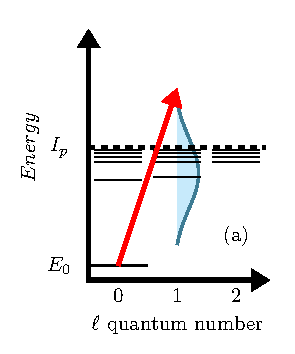
\includegraphics[width=.3\linewidth]{figs/Photo_ionization/short_pulse/scheme_1-photon.pdf}
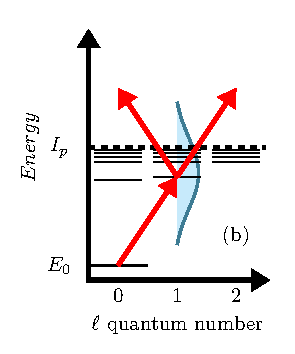
\includegraphics[width=.3\linewidth]{figs/Photo_ionization/short_pulse/scheme_2-photon.pdf}
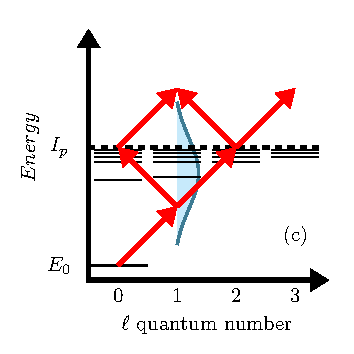
\includegraphics[width=.36\linewidth]{figs/Photo_ionization/short_pulse/scheme_3-photon.pdf}
\caption{
Schematic representation of one- (a), two- (b), and three-photon (c) ionization in an ultrashort pulse. The Gaussian distribution shows the spectral width of the ultrashort pulse centered about the energy of the $2p$-state. The red arrows represent the photon absorption pathways, and the black lines depict some of the resonant structure of the helium atom. (Figure from \cite{venzke2020_ionization})
} 
  \label{fig:scheme_short}
\end{figure}

\subsubsection{\label{ssub:short_scheme}Impact of one-, two-, and three-photon processes in ultrashort pulses}
To first illustrate the impact of the one-, two- and three-photon ionization pathways on the emission of the photoelectron in ultrashort laser pulses, let us consider an emission induced by a pulse with central frequency $\omega_0$ tuned to the $1s-2p$ energy gap. The broad energy spectrum of an ultrashort Gaussian pulse is schematically depicted in the panels of Figure \ref{fig:scheme_short} centered about the energy of the $2p$-state. Absorption of two photons by an electron in the ground state at the central frequency $\omega_0$ (c.f., Figure \ref{fig:scheme_short}(b)) will lead to its emission at energy $E = 2\omega_0 - |E_{1s}|$. If the bandwidth of the pulse is broad enough (i.e., the pulse duration is sufficiently short) ionization of a photoelectron with the same photoelectron energy can occur via absorption of one photon with energy $2 \omega_0$ (c.f., Figure \ref{fig:scheme_short}(a)) or via absorption of three photons with energy $\frac{2}{3} \omega_0$ (c.f., Figure \ref{fig:scheme_short}(c)). We note that besides the two-photon and three-photon pathways with absorption of photons of equal energies, there exist more such pathways to a final photoelectron energy $E$ for absorption of photons with unequal energy as long as the sum of the photon energies is equal to $2 \omega_E$.

The occurrence of the one- and three-photon processes requires a broad spectral bandwidth of the pulse. That means, for long pulses we expect that only the two-photon ionization process is present. If the pulse is shortened to a few optical cycles, both the one- and three-photon channels become effective, since the probability of photon absorption at energies away from the central frequency increases. In the perturbative intensity regime the probability for a $n$-photon process scales as $I^n$, where $I$ is the intensity of the pulse. We therefore expect that at a given ultrashort pulse duration at low intensities the one-photon process dominates over the two-photon process in an ultrashort laser pulse. As the intensity increases, first the two-photon process should then become dominant, before at significantly higher intensities contributions from the three-photon process will become detectable. In this section, we mainly study the transition from one- to two-photon processes, while the influence of the three-photon process will be given minor attention. 

\begin{figure}[!ht]
\centering
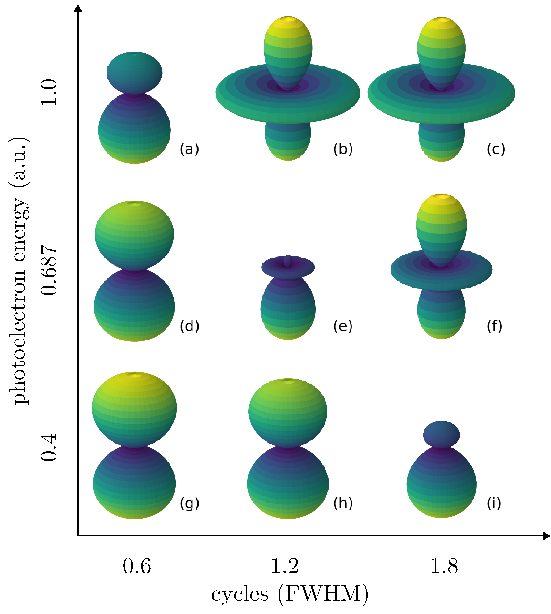
\includegraphics[width=0.5\linewidth]{figs/Photo_ionization/short_pulse/fig_1.eps}
\caption{
Photoelectron angular distributions for helium atom ionized by laser pulses at central photon energy $\omega_0 = 22.2$ eV, peak intensity $I_0 = 10^{11}$ W/cm$^2$, carrier-to-envelope phase $\phi = 0$ and three different pulse durations: $N = 0.6$ FWFM cycles (0.112 fs, left column), $N = 1.2$ FWHM cycles (0.224 fs, middle column) and $N = 1.8$ FWHM cycles (0.335 fs, right column). Angular distributions are obtained for three values of photoelectron energy $E = 1.45(2\omega_0 - |E_{1s}|) = 1.0$ a.u. (top row), $E = 2\omega_0 - |E_{1s}|$ = 0.687 a.u. (middle row), and $E = 0.58(2\omega_0 - |E_{1s}|) = 0.4$ a.u. (bottom row), where $E_{1s}$ is the energy of the $1s$ state in the SAE potential. (Figure from \cite{venzke2020_ionization})
} 
  \label{fig:pads}
\end{figure}

\subsubsection{\label{ssub:pads}One- vs. two-photon ionization}
In Figure \ref{fig:pads} we present examples of PADs that show the transition from single photon ionization, illustrated by the $p$-wave character of the distribution (panels (d, g, h)), to an emission following two-photon absorption, highlighted by the dominating $d$-wave character in the PAD (panels (b, c, f)). The results are obtained for ionization by a laser pulse at a central photon energy $\omega_0 = 22$ eV, which corresponds to the energy difference between the $1s$- and $2p$-states in the single-active electron potential for helium used in the calculations, peak intensity $I_0 = 10^{11}$ W/cm$^2$ and carrier-to-envelope phase $\phi = 0$. At a given photoelectron energy, the transition occurs for a variation of the pulse duration, e.g.\ at $E = 2\omega_0 - |E_{1s}|$ = 0.687 a.u. from 0.112 fs to 0.335 fs (middle row). Conversely, for a fixed pulse duration, the transition is seen for increase of the photoelectron energy, e.g.\ at $\tau = 0.224$ fs from 0.4 a.u. to 1.0 a.u. (middle column). In the transition regime the PADs exhibit the interference between the one- and two-photon ionization processes. 

\begin{figure}[!ht]
\centering
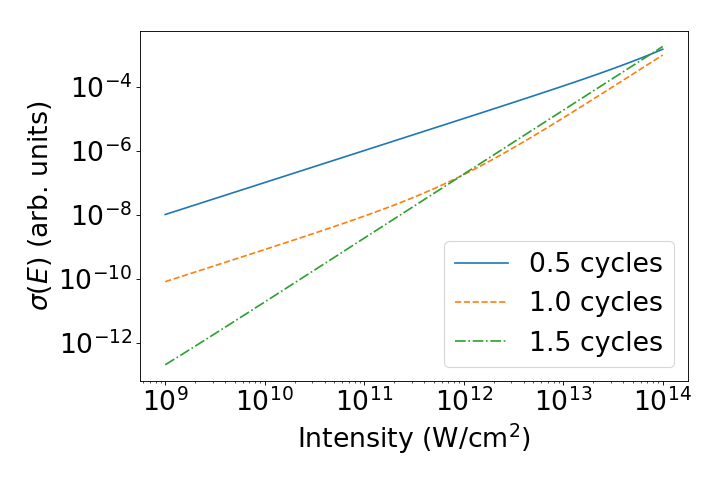
\includegraphics[width=0.49\linewidth]{figs/Photo_ionization/short_pulse/beta_0_cyc.png}\\
\caption{Cross section $\sigma(E)$ as a function of peak intensity for photoelectron emission at energy $E = 2\omega_0 - I_p = 18.7$ eV in 0.5-cycle (one-photon process dominates), 1.0-cycle (transition regime), and 1.5-cycle (two-photon process dominates). Central photon energy $\omega_0 = |E_{2p} - E_{1s}| = 22.2$ eV and carrier-to-envelope phase $\phi=0$.  (Figure from \cite{venzke2020_ionization})
} 
  \label{fig:cross}
\end{figure}

Further insights in the transition between the two processes can be found via the cross section $\sigma(E)$
and the first four anisotropy parameters $\beta_i$ ($i = 1, \ldots, 4$) . In Figure \ref{fig:cross} the results for the cross section are shown as function of peak intensity at fixed photon and photoelectron energies. The cross section for a 0.5 cycle pulse has a slope of one corresponding to the dominance of one photon ionization over the whole intensity regime. In contrast, the cross section obtained for the 1.5 cycle pulse is dominated by the two photon process due to the reduced bandwidth of the pulse. In the data for the 1-cycle pulse the transition from the one- to the two-photon process is seen to occur near 10$^{12}$ W/cm$^2$. 

\begin{figure}[!ht]
\centering
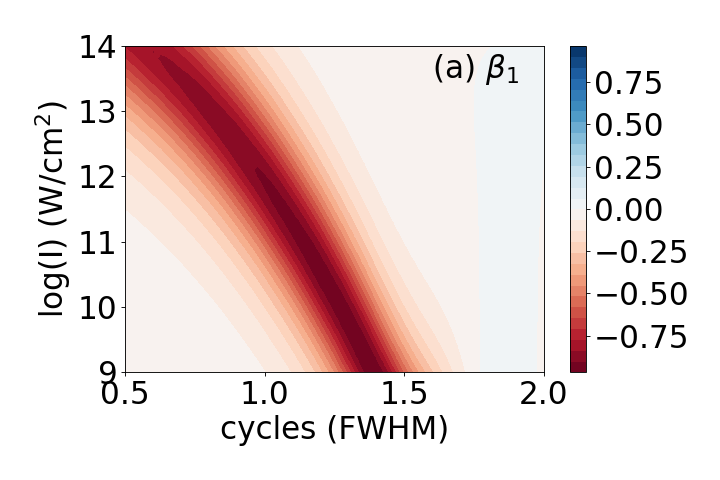
\includegraphics[width=0.49\linewidth]{figs/Photo_ionization/short_pulse/beta_1_heat.png}
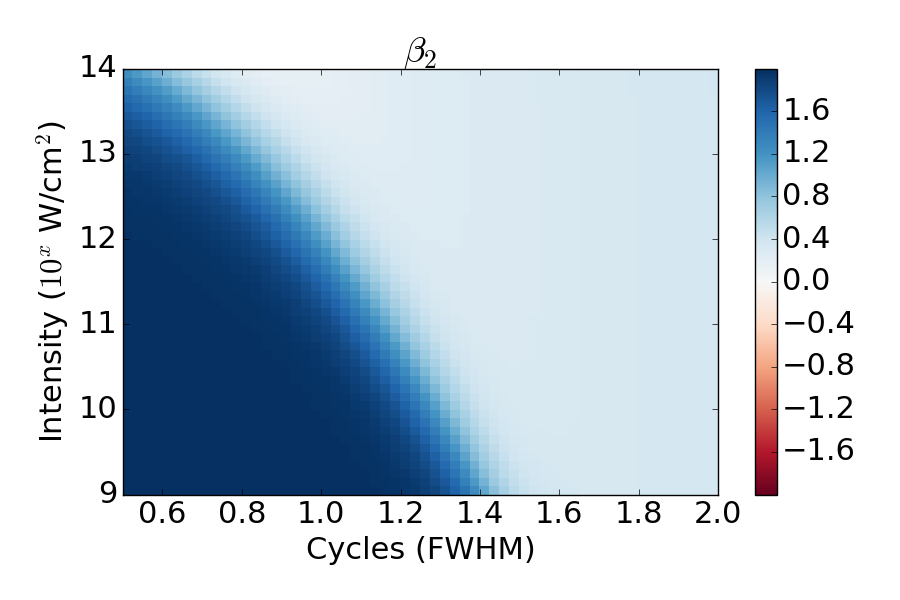
\includegraphics[width=0.49\linewidth]{figs/Photo_ionization/short_pulse/beta_2_heat.png}\\
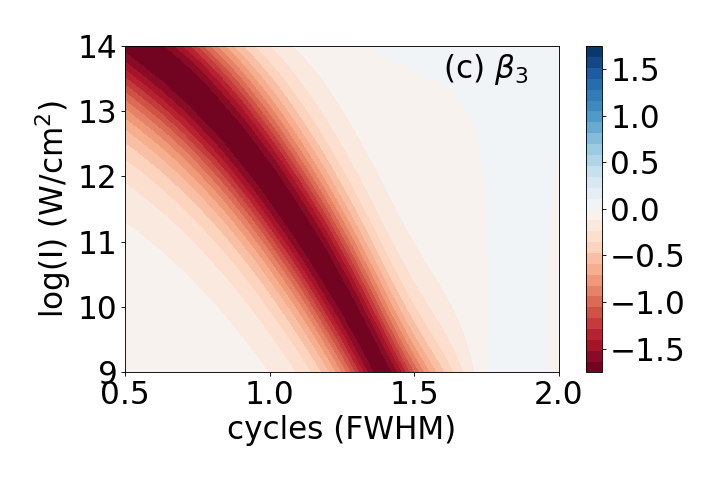
\includegraphics[width=0.49\linewidth]{figs/Photo_ionization/short_pulse/beta_3_heat.png}
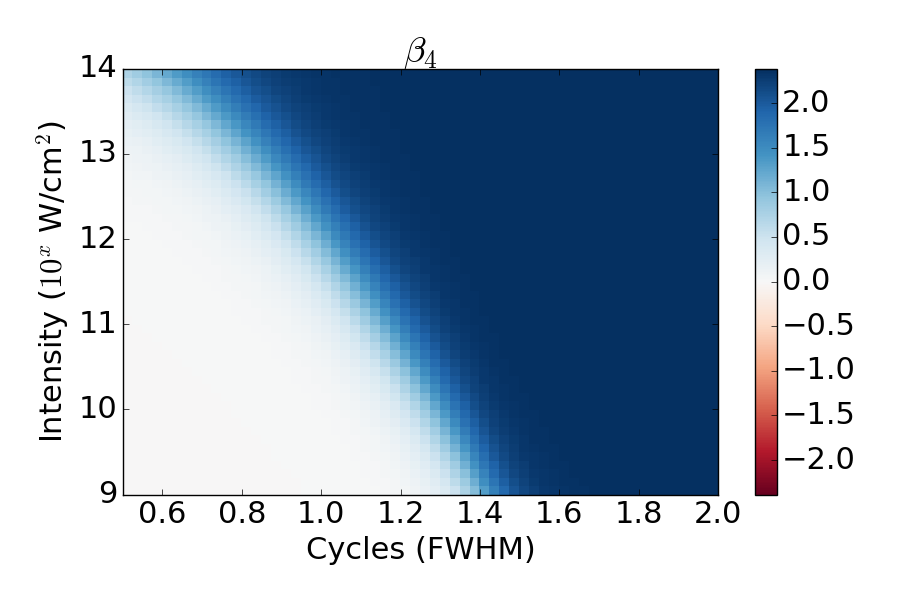
\includegraphics[width=0.49\linewidth]{figs/Photo_ionization/short_pulse/beta_4_heat.png}
\caption{
Parameters $\beta_1$ (a) to $\beta_4$ (d) as function of pulse duration (FWHM) and peak intensity. Central photon energy $\omega_0 = |E_{2p} - E_{1s}| = 22.2$ eV, carrier-to-envelope phase $\phi=0$ and photoelectron energy $E = 2\omega_0 - I_p = 18.7$ eV. (Figure from \cite{venzke2020_ionization})
} 
  \label{fig:beta}
\end{figure}

In Figure \ref{fig:beta} the results for the \textbf{$\beta$}-parameters are shown as function of pulse duration and peak intensity at fixed photon and photoelectron energies. The even $\beta$-parameters show the transition from dominant one-photon ionization ($\beta_2 > 0$, $\beta_4 \approx 0$) to dominant two-photon ionization ($\beta_2 \approx 0$, $\beta_4 > 0$), while the odd $\beta$-parameters exhibit the regime of interference between the two processes ($\beta_1 < 0$ and $\beta_3 < 0$ for $\phi=0$). The latter peak where the magnitudes of the two transition amplitudes coincide. At a given peak intensity the interference regime extends over a change of pulse duration of about 0.5 cycles at FWHM. For a fixed pulse duration, the interference regime extends over a variation of peak intensity by a factor of 2-5. We can therefore expect that the results are rather stable with respect to intensity fluctuations of the pulse. The impact of other potential pulse fluctuations in the experiment on the $\beta$-parameters will be discussed in subsection
\ref{ssub:variation}.

The transition probabilities of the one- and two-photon processes, $\sigma_1$ and $\sigma_2$, scale linearly and quadratically with intensity. Assuming that the two-photon ionization process involves predominantly the absorption of photons at equal energies, the peak intensity at maximum interference can be estimated as $I_{infer} \propto D^{(1)}(E)f(\Omega)/(D^{(2)}(E)f^2(\omega))$, where $D^{(i)}(E)$ is the square of the transition dipole moments for the one- and two-photon process, $f$ is the spectral distribution of the pulse and $\Omega = 2\omega = E + |E_{1s}|$. Since $\omega = \omega_0$ for the results in Figure \ref{fig:beta}, $f(\omega) = f(\omega_0) = 1$ and $I_{infer} \propto f(\Omega)$. Thus, we expect that the interference between the two processes requires a larger spectral bandwidth, i.e. shorter pulse duration, the larger the peak intensity of the pulse. The results in Figure \ref{fig:beta} confirm this expectation.

\begin{figure}[!ht]
\centering
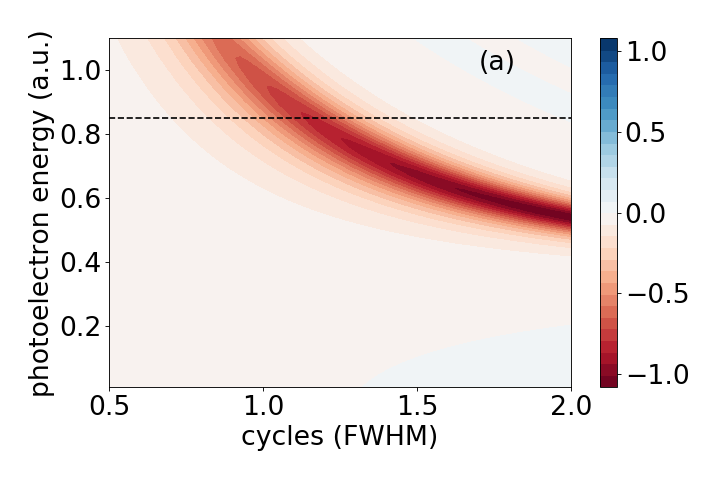
\includegraphics[width=0.40\linewidth]{figs/Photo_ionization/short_pulse/energy_d1p1_beta_1_I_1_heat.png}
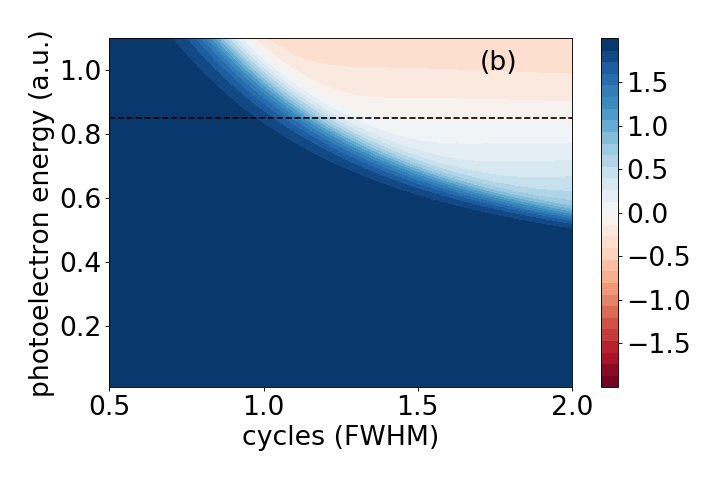
\includegraphics[width=0.40\linewidth]{figs/Photo_ionization/short_pulse/energy_d1p1_beta_2_I_1_heat.png}\\
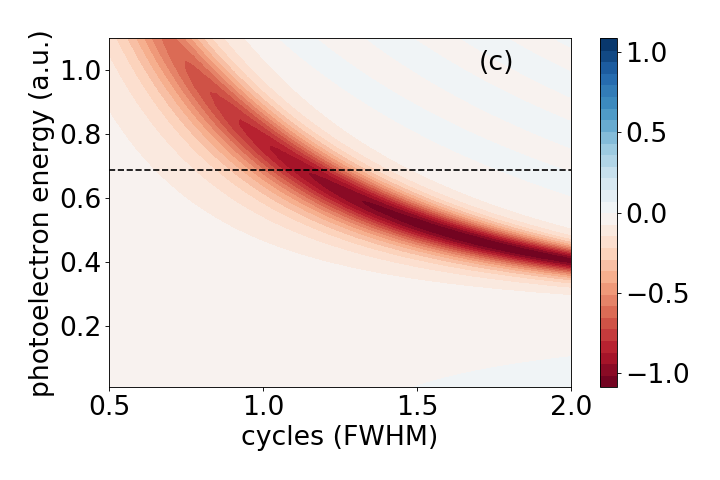
\includegraphics[width=0.40\linewidth]{figs/Photo_ionization/short_pulse/energy_d1p0_beta_1_I_1_heat.png}
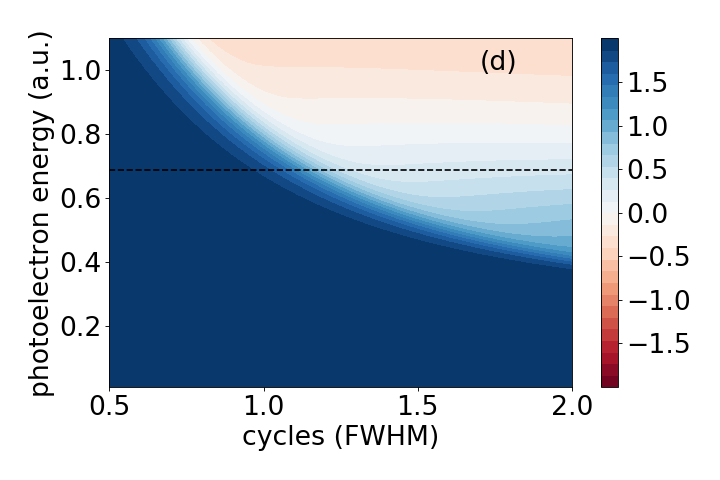
\includegraphics[width=0.40\linewidth]{figs/Photo_ionization/short_pulse/energy_d1p0_beta_2_I_1_heat.png}\\
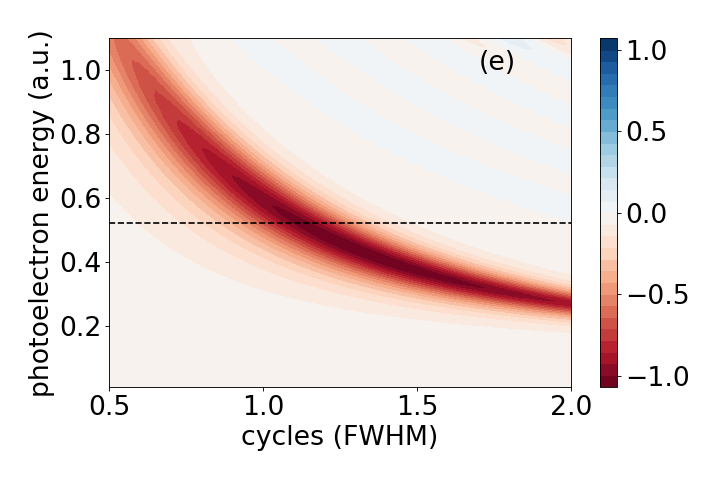
\includegraphics[width=0.40\linewidth]{figs/Photo_ionization/short_pulse/energy_d0p9_beta_1_I_1_heat.png}
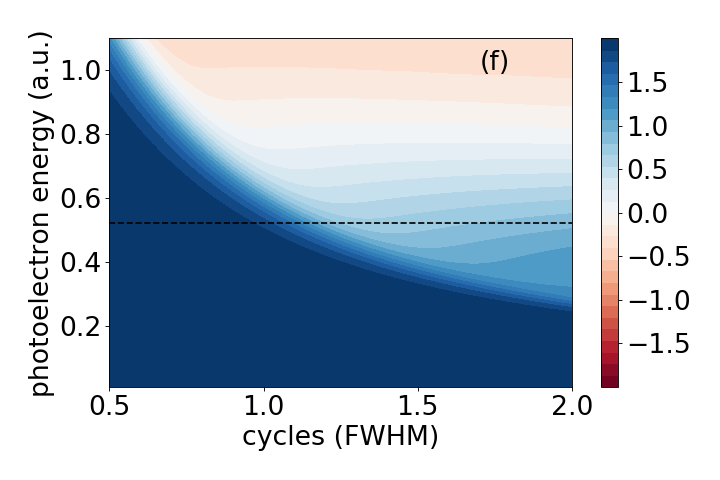
\includegraphics[width=0.40\linewidth]{figs/Photo_ionization/short_pulse/energy_d0p9_beta_2_I_1_heat.png}\\
\caption{
Anisotropy parameters $\beta_1$ (left) and $\beta_2$ (right) as function of pulse duration and photoelectron energy $E$ for central frequencies $\omega_0 = 1.1 |E_{1s}-E_{2p}|$ (top row), $\omega_0 = |E_{1s}-E_{2p}|$ (middle row) and $\omega_0 = 0.9 |E_{1s}-E_{2p}|$ (bottom row) at peak intensity of $10^{11}$ W/cm$^2$ and $\phi = 0$. In each panel the dashed line corresponds to $E = 2\omega_0 - I_p$.  (Figure from \cite{venzke2020_ionization})
} 
  \label{fig:beta_omega}
\end{figure}

Next, we consider how the transition between the two pathways depends on the photoelectron energy and the central photon frequency at a given peak intensity $I_0 = 10^{11}$ W/cm$^2$ and carrier-to-envelope phase $\phi = 0$. To this end, we show in the Figure \ref{fig:beta_omega} the 
anisotropy parameters $\beta_1$ (left column) and $\beta_2$ (right column) as a function of photoelectron energy and pulse duration for central frequencies below (top row), on (middle row) and above (bottom row) resonance with the $1s - 2p$ transition in the helium single-active electron potential. We restrict ourselves to $\beta_1$ and $\beta_2$ since the higher order $\beta$-parameters contain equivalent information (see Figure \ref{fig:beta}). Also shown in Figure \ref{fig:beta_omega} is the photoelectron energy $E = 2\omega_0 - I_p$, corresponding to a two-photon transition at the central frequency $\omega_0$. 

The comparison shows that the transition regime depends on the central frequency, since the regime shifts for a given pulse duration to larger photoelectron energies as the central frequencies increases (from bottom to top). At a given central frequency, the pulse duration, at which the transition between the one- and two-photon ionization pathways occurs, increases as the photoelectron energy decreases. Qualitatively, this dependence can be understood using the relation $I_{infer} \propto D^{(1)}(E)f(\Omega)/(D^{(2)}(E)f^2(\omega))$. For photoelectron energies larger than $E = 2\omega_0 - I_p$ (dashed line), both $\omega$ and $\Omega$ are larger than the central frequency. Consequently, at large photoelectron energies a broader spectral distribution (shorter pulse duration) is required for the same value of $f(\Omega)/f^2(\omega)$ than at photoelectron energies below $E = 2\omega_0 - I_p$ (dashed line), where $\omega < \omega_0$ while $\Omega > \omega_0$. 

\begin{figure}[!ht]
\centering
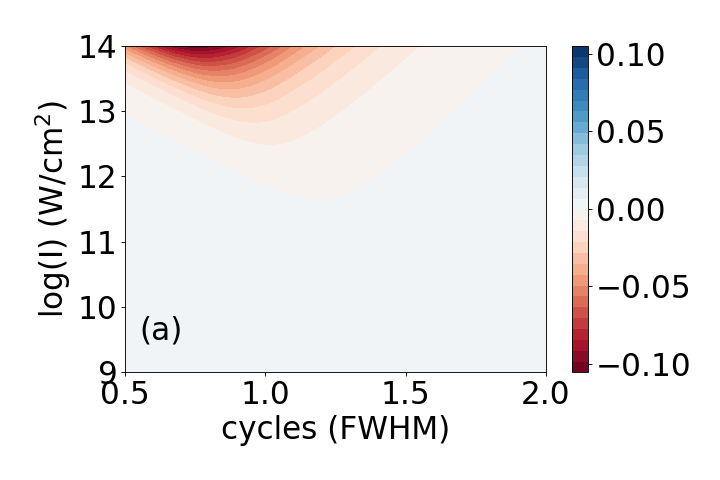
\includegraphics[width=0.4\linewidth]{figs/Photo_ionization/short_pulse/beta_5_heat.png}
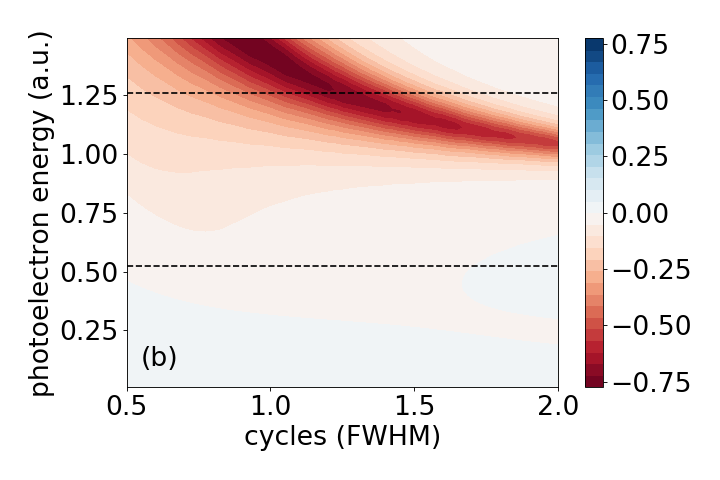
\includegraphics[width=0.4\linewidth]{figs/Photo_ionization/short_pulse/energy_d0p9_beta_5_I_2_heat.png}\\
\caption{
Anisoptropy parameter $\beta_5$ (a) as function of pulse duration and peak intensity at central frequency $\omega_0 = |E_{1s}-E_{2p}|$ and photoelectron energy $2\omega_0 - |E_{1s}|$ and (b) as function of pulse duration and photoelectron energy at central frequency $\omega_0 = 0.9|E_{1s}-E_{2p}|$ and peak intensity of $10^{13}$ W/cm$^2$. The dotted lines correspond to $E = 2\omega_0 - I_p$ and $E = 3\omega_0 - I_p$. The other parameters are as in Figures \ref{fig:beta} and \ref{fig:beta_omega}, respectively. (Figure from \cite{venzke2020_ionization})
} 
  \label{fig:beta-3w}
\end{figure}

Finally, we briefly mention that in the limit of short pulses and high intensities, both the one- and three-photon processes can interfere since the three-photon process scales with $I^3$. The results for the anisotropy parameter $\beta_5$ in Figure \ref{fig:beta-3w} confirm this expectation. At a photoelectron energy of $2\omega_0 - |E_{1s}|$ (panel (a)) a peak intensity of about $10^{14}$ W/cm$^2$ and a rather large spectral bandwidth is required to facilitate the three-photon process with significant probability since the corresponding photon energies are smaller than the central frequency. The distribution over photoelectron energy (panel (b)) shows that the impact of the three-photon ionization process is indeed more visible at energies near $E = 3\omega_0 - |E_{1s}|$.

\subsubsection{\label{ssub:variation} Impact of pulse fluctuations}
For the discussion in the previous subsection we have considered results obtained at fixed pulse parameters. The results in Figures \ref{fig:beta} and \ref{fig:beta_omega} show that the transition regime occurs over a rather small window of pulse duration while it appears to be rather stable for variations of the peak intensity up to half an order of magnitude. The photon energies in the extreme ultraviolet can be nowadays generated using high-order harmonics or free electron lasers. In view of the technical difficulties to control the carrier-to-envelope (CEP) of ultrashort pulses as well as the fluctuating pulse shapes in the self-amplified spontaneous emission (SASE) mode of free electron lasers, we have studied the impact of these variations on the anisotropy parameters. 

\begin{figure}[!ht]
\centering
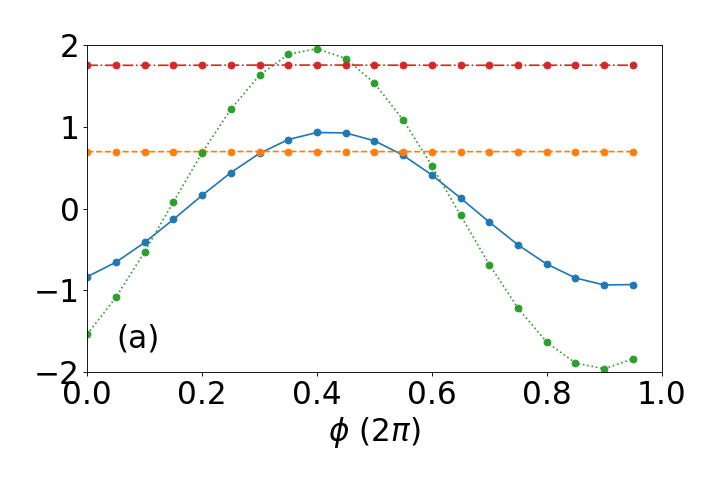
\includegraphics[width=0.32\linewidth]{figs/Photo_ionization/short_pulse/Beta_vs_cep.png}
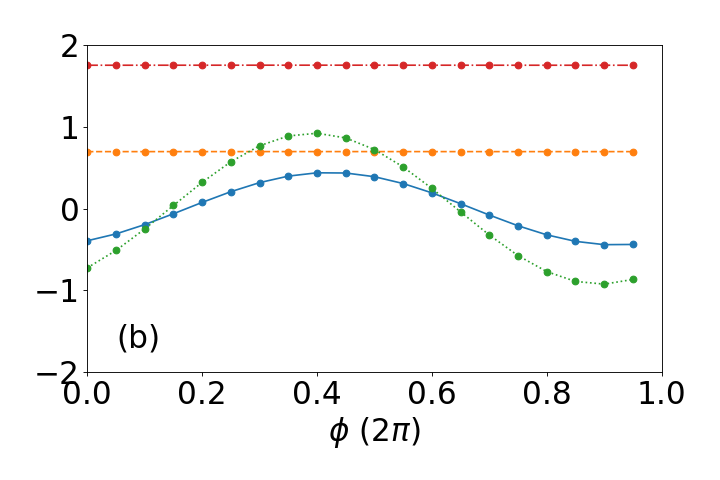
\includegraphics[width=0.32\linewidth]{figs/Photo_ionization/short_pulse/Beta_vs_cep_0p20.png}
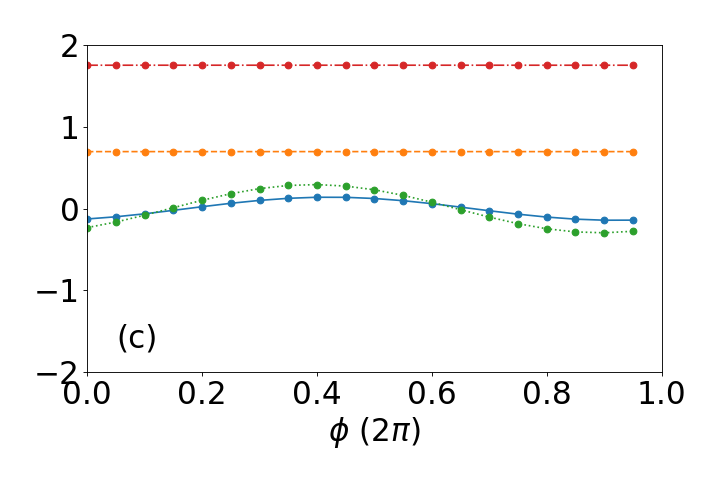
\includegraphics[width=0.32\linewidth]{figs/Photo_ionization/short_pulse/Beta_vs_cep_0p40.png}
\caption{
Anisotropy parameters $\beta_1$ (solid line), $\beta_2$ (dashed line), $\beta_3$ (dotted line) and $\beta_4$ (dashed-dotted line) as function of carrier-envelope-phase. The results averaged using a Gaussian distribution for the CEP (c.f., Eq.\ (\ref{eq:gauss_window})) with widths of (b) $\alpha = 0.2$ (in units of $2\pi$) and (c) $\alpha = 0.4$ are compared with the unaveraged results (a). Peak intensity: $10^{11}$ W/cm$^2$, central frequency:  $\omega_0 = |E_{1s}-E_{2p}|$, pulse duration: 1.2 FWHM cycles and photoelectron energy $2\omega_0 - |E_{1s}|$. (Figure from \cite{venzke2020_ionization})
} 
  \label{fig:beta_cep}
\end{figure}

To study the dependence on the CEP we have averaged the results about a given value $\phi_0$ using a Gaussian distribution of width $\alpha$ as: 
%
\begin{equation}
\beta_j^{(\alpha)}(\phi_0) 
= 
\frac{\sum_i \exp\left[-\frac{1}{2}\left(\frac{|\phi_i-\phi_0|}{2\pi\alpha}\right)\right] \sigma(\phi_i) \beta_j(\phi_i)}
{\sum_i\exp\left[-\frac{1}{2}\left(\frac{|\phi_i-\phi_0|}{2\pi\alpha}\right)\right] \sigma(\phi_i)}\; ,
    \label{eq:gauss_window}
\end{equation}
%
where $\sigma(\phi_i)$ is the total ionization probability at CEP $\phi_i$. The results for averages with (b) $\alpha = 0.2$ and (c) $\alpha = 0.4$ are compared in Figure \ref{fig:beta_cep} with the unaveraged results (panel (a)). As expected, the odd $\beta$-parameters, which reflect the interference between the one- and two-photon processes, strongly depend on CEP, while the even parameters are independent of it. Thus, the transition from one-photon to two-photon ionization can be observed via $\beta_2$ and $\beta_4$ even in pulses without CEP stabilization. Although the odd parameters depend on CEP, the corresponding results appear to be indicative for the transition up to fluctuations of about $\pi/2$.

We have further studied the impact of fluctuations of temporal FEL laser pulse shapes \cite{mitzner2008}. We note that current FEL technology does not provide the bandwidth required to generate pulses down to the one- or two-cycle limit at the photon energies considered here. We may still attempt to give some theoretical insights concerning the robustness of the signal against the major fluctuations present in an FEL pulse. To this end, we have applied a partial coherence method, which has been used before to model longer FEL pulses \cite{pfeiffer2010}. We note that future technological progress towards generation of ultrashort FEL pulses in the EUV regime may necessitate to extent the current approach.

To generate the FEL pulses used in the numerical simulations, the spectrum of a vector potential with Gaussian envelope corresponding to peak intensity $I_0$ and FWHM pulse duration $\tau_0$ is used as an input. Each spectral component is then multiplied with a random phase factor and an inverse Fourier transform is taken producing $A'(t)$, which is then normalized and windowed in time to give:
\begin{equation}
    A_{FEL}(t) = A_0 f(t)\frac{Re\left[A'(t)\right]}{\max|Re\left[A'(t)\right]|}
\end{equation}
where $A_0=c E_0/\omega_A$ in Equation (\ref{eq:vectorp}) and $f(t)$ represents the envelope, here a Gaussian envelope. The electric field of the FEL pulse is then obtained using Equation (\ref{eq:efield}). The resulting pulse simulates the partially coherent nature of the SASE pulses produced by an FEL. 
The average of results from numerical simulations over an increasing number of shots is expected to resemble results similar to those produced during an FEL beam-time. Here, the $\beta$-parameters are calculated using a weighted average
% 
\begin{equation}
\beta_j^{FEL}(E) 
= 
\frac{\sum_i^{N_{shots}}  \sigma_i(E) \beta_{j,i}(E)}
{\sum_i^{N_{shots}}\sigma_i(E)}\; ,
    \label{eq:FEL_beta}
\end{equation}
% 
to account for the photoelectron yield shot to shot.

\begin{figure}[!ht]
\centering
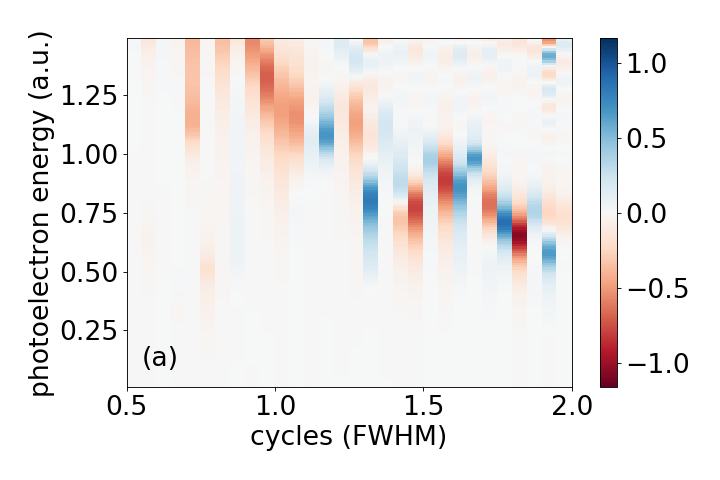
\includegraphics[width=0.4\linewidth]{figs/Photo_ionization/short_pulse/Beta_1_FEL_1_shot.png}
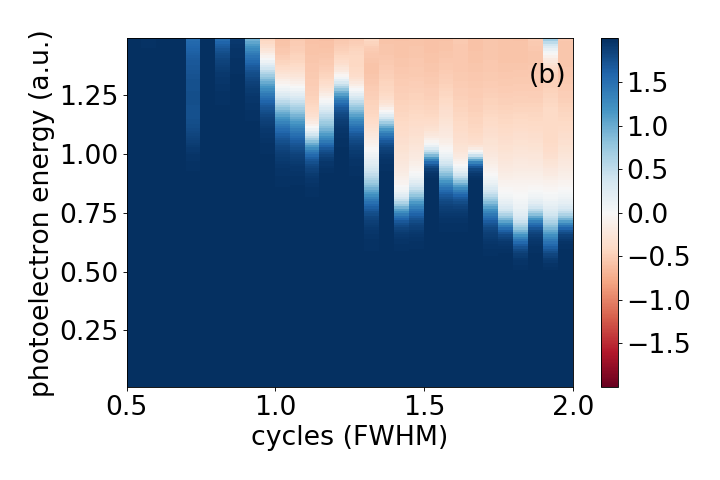
\includegraphics[width=0.4\linewidth]{figs/Photo_ionization/short_pulse/Beta_2_FEL_1_shot.png}\\
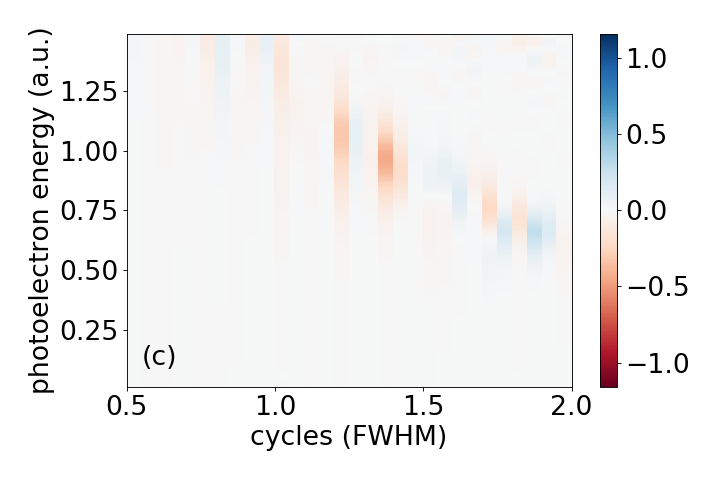
\includegraphics[width=0.4\linewidth]{figs/Photo_ionization/short_pulse/Beta_1_FEL_10_shot.png}
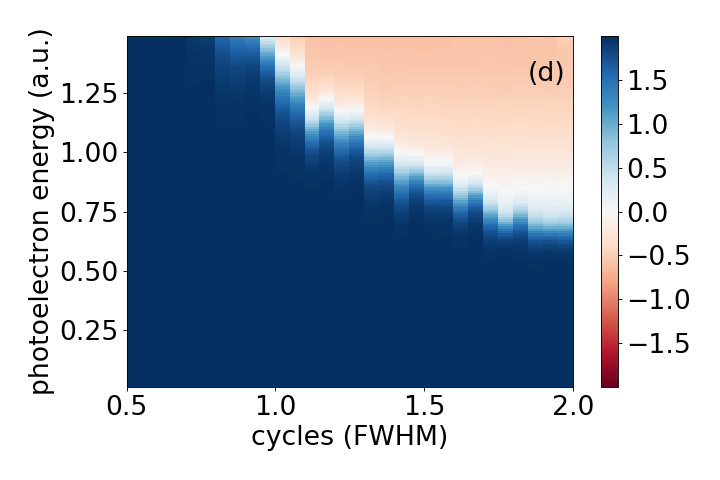
\includegraphics[width=0.4\linewidth]{figs/Photo_ionization/short_pulse/Beta_2_FEL_10_shot.png}\\
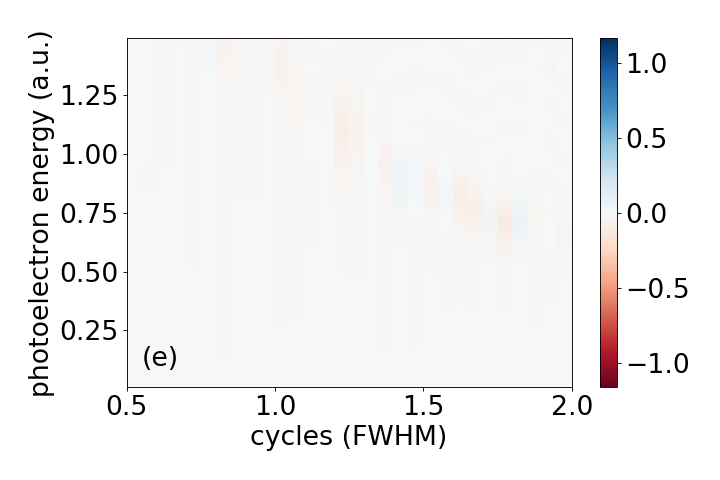
\includegraphics[width=0.4\linewidth]{figs/Photo_ionization/short_pulse/Beta_1_FEL_200_shot.png}
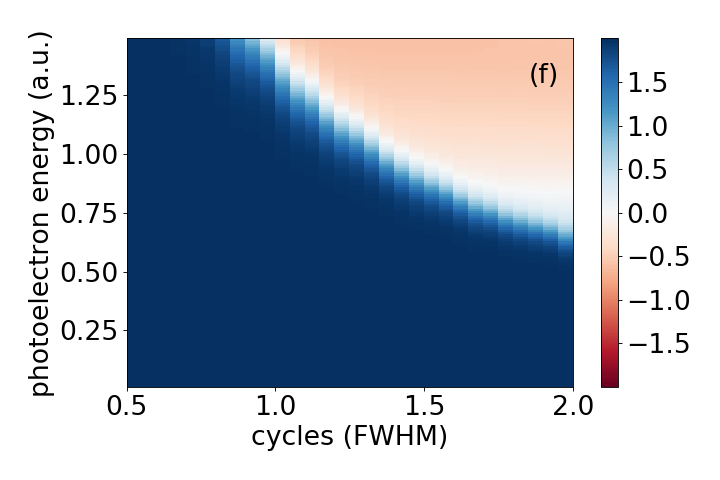
\includegraphics[width=0.4\linewidth]{figs/Photo_ionization/short_pulse/Beta_2_FEL_200_shot.png}
\caption{
Anisotropy parameters $\beta_1$ (left) and $\beta_2$ (right) as function of pulse duration of the Gaussian window used in modeling the FEL pulses and photoelectron energy averaged over 10 (middle row) and 200 (bottom row) partially incoherent free electron pulses as compared to a single shot result (top row). Peak intensity of the Gaussian window: $I_{0} = 10^{11}$ W/cm$^2$ 
and central frequency of the spectral distribution $\omega_0 = |E_{1s}-E_{2p}|$. (Figure from \cite{venzke2020_ionization})
} 
  \label{fig:beta-variation-FEL}
\end{figure}

In Figure \ref{fig:beta-variation-FEL} we compare the results for $\beta_1^{FEL}$ (left) and $\beta_2^{FEL}$ (right) as function of photoelectron energy and pulse duration of the Gaussian window used in modeling the FEL pulses, averaged over 10 (panels (c, d)) and 200 (panels (e, f)) FEL shots for each pulse length (i.e., 6,200 calculations in total) with the exemplary results from a single shot (panels (a,b)). A robust distribution for $\beta_2^{FEL}$ emerges as the number of shots increases, clearly showing the transition from a one- to a two-photon process (the same conclusion holds for $\beta_4^{FEL}$, not shown). However, the interference in the photoelectron angular distributions cannot be determined via FEL laser pulses, since the results for $\beta_1^{FEL}$ and $\beta_3^{FEL}$ (not shown) average to zero in the transition regime. 
We note that the generated FEL pulses are not transform-limited and the pulse duration of the Gaussian window used in modeling the pulses does not correspond to that of Gaussian pulses used in the previous subsection
\ref{ssub:pads}.
Comparing the data presented in Figure \ref{fig:beta-variation-FEL}(f) with those in Figure \ref{fig:beta_omega}(d) we estimate that the effective pulse duration of a bandwidth-limited Gaussian pulse with a spectrum corresponding to the average spectrum of the generated FEL pulses is about 0.6 times shorter than that of the Gaussian window.

\subsection{Summary}
In this Section we have provided theoretical results, obtained from numerical solutions of the time-dependent Schr\"odinger equation, for the competition between one-photon and two-photon ionization in an ultrashort extreme-ultraviolet laser pulse. We have shown that the transition between the two processes can be observed in the photoelectron angular distributions and the related anisotropy parameters $\beta_i$ ($i = 1, \ldots 4$) as function of pulse duration, peak intensity, central photon frequency and photoelectron energy distribution. While the even $\beta$-parameters exhibit the transition via a change from zero to a finite value, the odd parameters indicate the interference regime. At given photon and photoelectron energies this regime extends over about 0.5 FWHM cycles in duration and a variation by a factor of 2-5 in peak intensity. The impact of three-photon ionization, which becomes available at these broadband pulses as well, is seen at high intensities and large photoelectron energies. Finally, we have considered typical variations in the CEP of ultrashort pulses, e.g. as produced in high harmonic generation, and fluctuating pulse shapes in free-electron laser pulses. It is found that the transition between one- and two-photon ionization can be observed via the even $\beta$-parameters in FEL pulses and pulses without CEP stabilization.
% section short_pulse_effect (end)


%%%%%%%%%%%%%%%%%%%%%%%%%%%%%%%%%%%%%%%%%%%%%%%%%%%%%%%%%%%%%%%%%%%%%%%%%%%%%%%%%%%%%%%%%%%%%%%%%%%%%%%%%%%%%%%%%%
%%%%%%%%%%%%%%%%%%%%%%%%%%%%%%%%%%%%%%%%%%%%%%%%%%%%%%%%%%%%%%%%%%%%%%%%%%%%%%%%%%%%%%%%%%%%%%%%%%%%%%%%%%%%%%%%%%
%%%%%%%%%%%%%%%%%%%%%%%%%%%%%%%%%%%%%%%%%%%%%%%%%%%%%%%%%%%%%%%%%%%%%%%%%%%%%%%%%%%%%%%%%%%%%%%%%%%%%%%%%%%%%%%%%%
%%%%%%%%%%%%%%%%%%%%%%%%%%%%%%%%%%%%%%%%%%%%%%%%%%%%%%%%%%%%%%%%%%%%%%%%%%%%%%%%%%%%%%%%%%%%%%%%%%%%%%%%%%%%%%%%%%
%%%%%%%%%%%%%%%%%%%%%%%%%%%%%%%%%%%%%%%%%%%%%%%%%%%%%%%%%%%%%%%%%%%%%%%%%%%%%%%%%%%%%%%%%%%%%%%%%%%%%%%%%%%%%%%%%%
\section[Generalized asymmetry parameters]{Generalized asymmetry parameters\protect\footnote{The content of this section has been also published in J. Venzke et al., Sci. Rep. \textbf{10}, 16164 (2020).}} % (fold)
\label{sec:generalized_asymmetry_parameters}



% Ultrabright light sources such as free-electron lasers \cite{seddon2017} and table-top laser systems based on high-order harmonic generation \cite{popmintchev2010,chini2014} deliver high-intensity pulses of few- or sub-femtosecond duration. Nowadays, laser pulses with a duration of a few tens of attoseconds have been achieved experimentally \cite{zhao2012,chen2014}. Isolated attosecond pulses or trains of attosecond pulses have been generated from the vacuum ultraviolet to the soft X-ray wavelength regime and the polarization of such pulses can nowadays be controlled. This recent progress in ultrafast laser pulse technology makes it possible to probe, steer and control the dynamics of electrons in atoms, molecules and solids \cite{vrakking2014,pazourek2015,calegari2016,xu2016,ramasesha2016,peng2019}.
% To name a few examples, the time-resolved measurement of the electron emission in the photoelectric effect has been realized \cite{cavalieri2007,schultze2010,klunder2011, tao2016,isinger2017}. Using an isolated attosecond pulse or a train of extreme-ultraviolet attosecond pulses to ionize an atom along with an infrared laser field interferograms have been measured to obtain information about phases of electron wavepackets, an important milestone towards reconstructing the wavefunctions of atoms \cite{remetter2006,mauritsson2010}. By extracting the phase and amplitude via application of photoelectron spectroscopy recently the birth of a photoelectron through a Fano resonance has been observed on the attosecond time scale \cite{gruson2016}.

% Probing atoms and molecules in their ground or excited states with ultrashort laser pulses opens a new regime where several linear and nonlinear ionization pathways compete and interfere \cite{ishikawa2012,ma2013,grum-grzhimailo2015,douguet2016,hofbrucker2018,boll2019,wang2019,venzke2020_ionization}. For example, it has been shown how the competition between resonant and nonresonant pathways depends on the pulse width \cite{ishikawa2012}. An important observable are photoelectron angular distributions (PAD), which are measured by detecting the probability for emission of the electron from the target in different directions. Since PADs are determined by the amplitudes and phases of the partial waves of all pathways contributing to the emission, they are practical means to identify the different contributing pathways. A characteristic signature of such interferences are asymmetries in the emission of the photoelectron \cite{yin1992}. In the simple case of photoionization from a single state, anisotropy and asymmetry parameters have been used in the past to identify and analyze interesting physical effects. A significant circular dichroism via the asymmetry in the forward-backward electron emission from bromocamphor molecules induced by circularly polarized light has been identified  \cite{bowering2001}. Observation of the breakdown of the symmetry in the photoelectron emission of argon has been shown in the region of the Cooper minimum \cite{ilchen2018}. Interferences between resonant and non-resonant pathways \cite{ishikawa2012} or direct and autoionizing channels \cite{cirelli2018} can be identified via anisotropy and asymmetry parameters. Other examples can be found in double photoionization \cite{maulbetsch1992} or molecular vibrations and chirality \cite{garcia2013} and applications range from studies of coherent control \cite{prince2016} to the characterization of ultrashort laser pulses \cite{chelkowski2002}.

While studies of quantum systems in a single state are important, very interesting physics arises from the systems in superposition states. Nowadays the most prominent example of a two-level quantum mechanical system is a qubit with its important applications in quantum computation and quantum simulations \cite{saffman2016}. Yet, also the internal motion of quantum mechanical systems, whether it is rotational, vibrational or electronic, is determined via superposition states. In ultrafast science the observation and resolution of such dynamics and, hence, the observation of atoms or molecules in superposition states has always played a central role. Currently, it is the superposition of atomic or molecular electronic states and the related attosecond electron dynamics that is the focus of studies in the field \cite{goulielmakis2010,mauritsson2010,holler2011,xie2012}. Perhaps the simplest case of such dynamics is a helium atom in a superposition of $1s$ and $2p_1$ state which results in a wavepacket rotating in a plane around the nucleus with a period of $\sim200$ attoseconds. The dynamics in such quantum systems in superposition states can be probed via ionization with an ultrashort laser pulse. Unlike for the ionization of a quantum system prepared in a single state, e.g. the ground state, conventional anisotropy and asymmetry parameters fail to provide comprehensive tools for the analysis of photoionization from atomic superposition states. As shown in the previous section, the simplest case of a competition between one- and two-photon ionization processes can be analyzed using asymmetry parameters if the atom is prepared in the ground state (see also,  \cite{ishikawa2012,ma2013,grum-grzhimailo2015,douguet2016,hofbrucker2018,boll2019,wang2019,venzke2020_ionization}). In contrast, these analysis tools are either not applicable or do not provide a straightforward interpretation for the same processes if the atom is in the superposition of two states. Thus, an extension of the toolbox for the characterization of the states and the identification of competing pathways is desirable. In this section, we propose a new set of generalized asymmetry parameters which are sensitive to interference effects in the photoionization of atomic systems in superposition states. As we will show these new parameters can be used to identify the interplay of competing linear and nonlinear pathways at low and high intensities, as well as at ultrashort pulse durations. The application and relevance of the parameters is tested using state-of-the-art numerical solutions of the time-dependent Schr\"odinger equation. Our method provides a new approach to the analysis of experiments dedicated to resolving attosecond electron dynamics.


\begin{figure}[!ht]
\begin{center}
    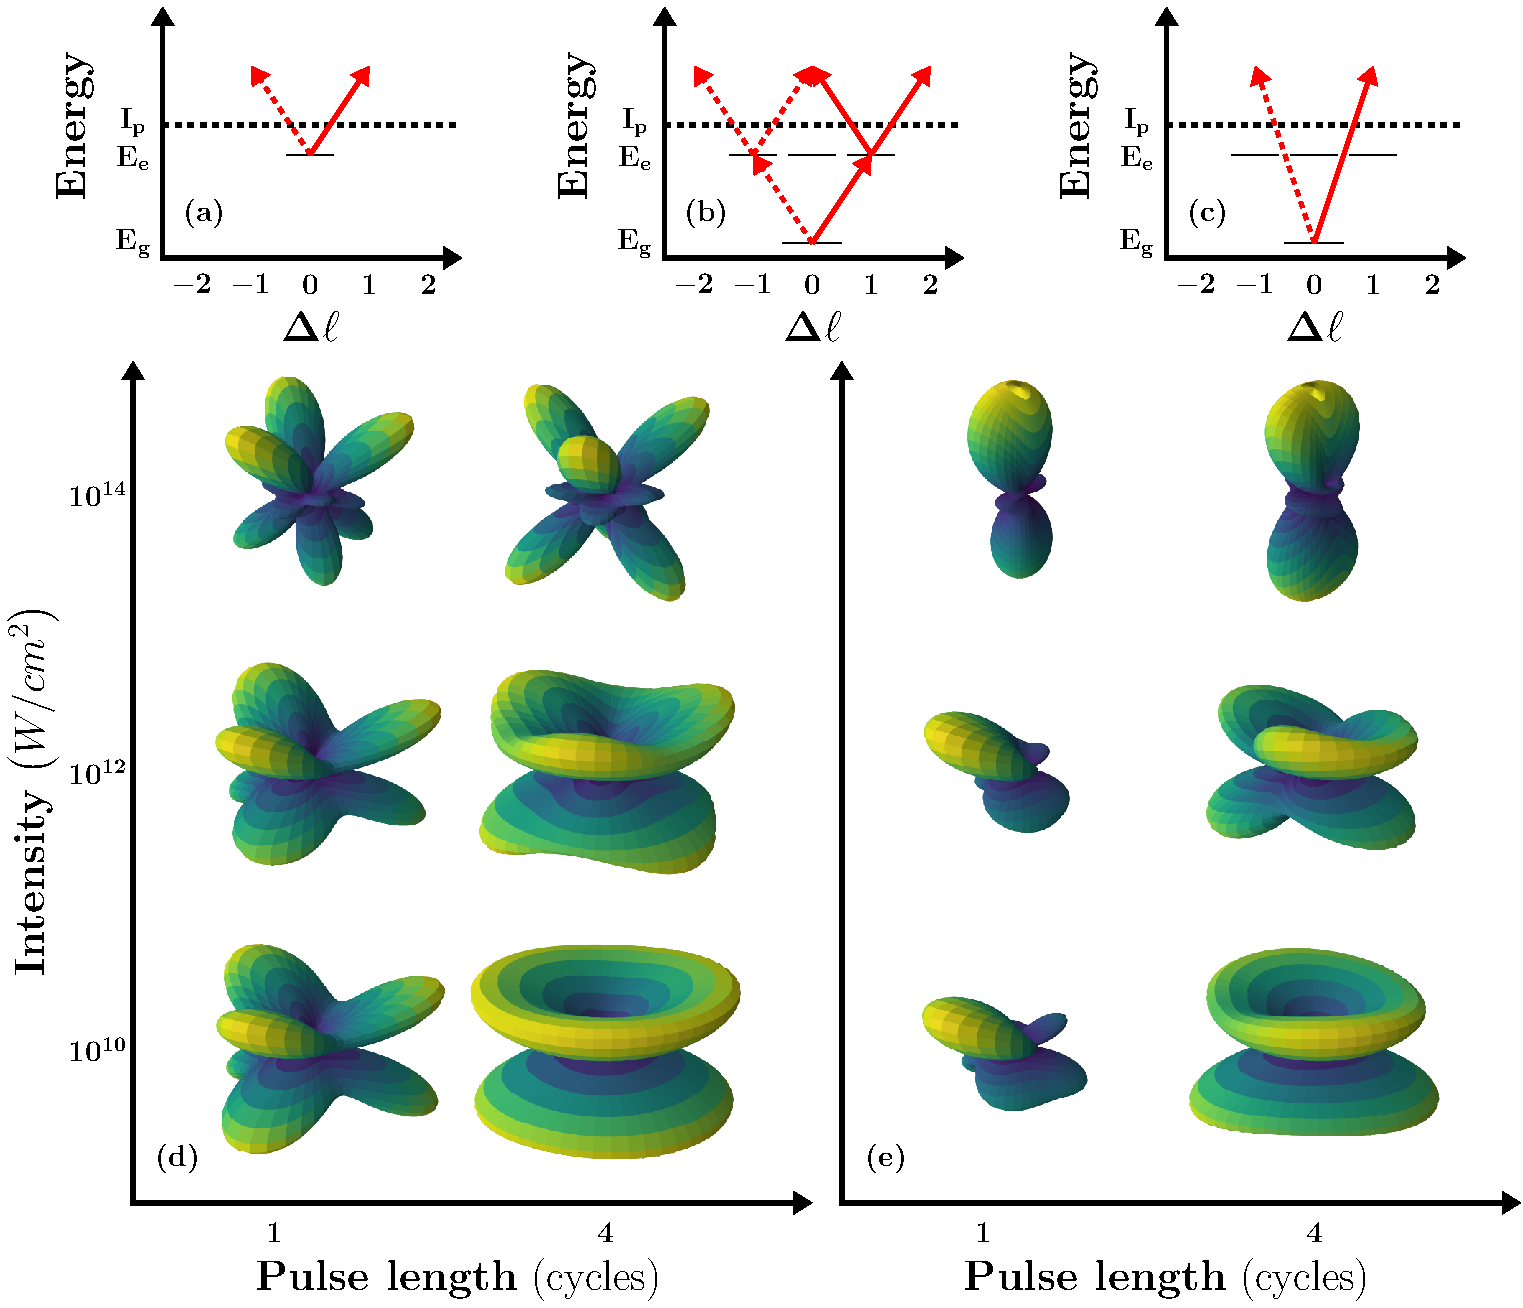
\includegraphics[width=0.9\linewidth]{figs/Photo_ionization/GAP/combine_fig_1.pdf}
\end{center}
\caption{
(a-c): Ionization pathways effective in different intensity and pulse length regimes. (d) Photoelectron angular distributions for ionization of neon atom, prepared in $2p_{-1}-3d_2$ superposition, as function of intensity and pulse length. (e) The same as (d) including additionally ionization from the $2p_0$ and $2p_1$ states. (Figure from \cite{venzke2020_GAP})
} 
  \label{fig:scheme_GAP_lin}
\end{figure}

\subsection{Generalized asymmetry parameters}
We consider a prototypical example in ultrafast science and, more general, in atomic physics, which is schematically shown in Fig.~\ref{fig:scheme_GAP_lin}. 
An atom in a superposition of two quantum states with different magnetic quantum numbers $m$, say the ground (g) and an excited (e) state is probed via ionization by an ultrashort linearly polarized laser pulse. The photoelectron emission is induced by a pulse with central frequency $\omega$ tuned to the energy gap of the two states. The broad energy spectrum of an ultrashort Gaussian pulse is schematically depicted in the panels of Fig.~\ref{fig:scheme_GAP_lin} centered about the energy of the excited state. There are three competing pathways leading to photoelectron emission with energy $2\omega - |E_g|$, where $E_g$ is the ground state energy of the atom: (a) absorption of one photon at $\omega$ from the
excited state, (b) absorption of two photons with sum frequency $2\omega$ from the 
ground state and (c) absorption of one photon at $2\omega$ from the ground state. While the ionization from the excited state (a) is the dominant pathway at low peak intensities and long pulse duration, the transitions from the ground state will interfere at higher peak intensities (two-photon process, (b)) and if the bandwidth of the pulse is broad enough (i.e., the pulse duration is sufficiently short, (c)). 
The exemplary results obtained from the solutions of the time-dependent Schr\"odinger equation in Fig.\ \ref{fig:scheme_GAP_lin} for the interaction of
neon atom, prepared in the superposition of $2p_{-1}$- and $3d_2$-states (d) or prepared in the same superposition but including additionally ionization from the $2p_0$ and $2p_1$ ground states (e), with a linearly polarized laser pulse show that the photoelectron angular distributions (PADs) vary significantly as function of pulse duration and peak intensity. 
The forward-backward asymmetry, often used in the past, cannot be applied to
identify the impact of the different pathways in these PADs. Therefore, a new set of asymmetry parameters is needed for photoionization from superposition states with ultrashort laser pulses.

\subsubsection{Definition}

We start by expanding the PAD as a coherent sum of spherical harmonics, assuming 
the atom is ionized by a linearly polarized pulse aligned along the $z$-axis as
\begin{equation}
    P(\theta,\phi) = \left|\sum_\ell C_{\ell}^{m_g} Y_\ell^{m_g}(\theta,\phi)+C_{\ell}^{m_e} Y_\ell^{m_e}(\theta,\phi)\right|^2
\end{equation}
where $m_g$ ($m_e$) are the magnetic quantum numbers of the ground (excited) state in the superposition, $C_\ell^m$ is the complex amplitude and $Y_\ell^m(\theta,\phi)$ is the spherical harmonic. The asymmetry in the PADs due to the interference between different channels is related to the relative phase and amplitude of the spherical harmonics. For each spherical harmonic, the sign of the phase is symmetric (asymmetric) across the $xy$-plane when $\ell+m$ is even (odd), while
in the $xy$-plane 
the phase is proportional to $e^{im\phi}$. 

In the $xy$-plane there are regions of destructive and constructive interference between the transition amplitudes from the ground and excited state, as illustrated on the left of Fig.~\ref{fig:integrals}. The regions can be labeled by
\begin{equation}
    c_i = \floor*{\frac{(\phi-\phi_0)\Delta m}{\pi}}
\end{equation}
where $\floor{}$ is the floor function, $\phi_0$ is a reference angle, and $\Delta m=|m_g-m_e|$ ($\Delta m = 3$ in Fig.~\ref{fig:integrals}). Setting $\phi_0$ at an angle where the interference switches from constructive to destructive, regions of destructive interference signal are labeled by even $c_i$ while odd $c_i$ denote regions of constructive interference. 
Next we define the following integrals:
\begin{align}
    I^{even}_{\pm} &= \sum_{even \; c_i} \int P(\theta,\phi)\; d\Omega_{c_i}^{\pm}\\
    I^{odd}_{\pm} &= \sum_{odd \; c_i} \int P(\theta,\phi)\; d\Omega_{c_i}^{\pm}
\end{align}
where $d\Omega_{c_i}$ is the solid angle for the region $c_i$ in the positive ($z>0$) or negative ($z<0$) hemisphere with respect to the $xy$-plane. In the example in Fig.~\ref{fig:integrals} (left) each integral represents the total photoelectron signal in the regions of a specific color (dark blue, light blue, dark red, light red). We now define general asymmetry parameters (GAPs) that account for the relative difference in the regions of constructive and destructive interference: 
\begin{equation}
\label{gaps}
    A_{p}^{\Delta m} \equiv \begin{cases} 
      \left|\frac{(I^{even}_+ + I^{even}_-) - (I^{odd}_++I^{odd}_-)}{I^{even}_++I^{even}_- + I^{odd}_++I^{odd}_-}\right|_{max(\phi_0)} & \text{even} \;  \gamma  \\ 
      \\
      \left|\frac{(I^{even}_++I^{odd}_-) - (I^{odd}_++I^{even}_-)}{I^{even}_++I^{even}_- + I^{odd}_++I^{odd}_-}\right|_{max(\phi_0)} & \text{odd} \;  \gamma 
  \end{cases}
\end{equation}
where $\gamma = \ell_e + m_e + \ell_g + m_g + N_p$ with $\ell_g$ ($\ell_e$) are the quantum numbers of the ground (excited) state in the superposition, and $p=(\gamma \text{ mod } 2)$ is the parity of $\gamma$. Each parameter $A_{p}^{\Delta m}$ is related to a certain total number of absorbed photons, $N_p = N_{g}+N_{e}$, where $N_g$ ($N_e$) is the number of photons absorbed in the transition from the ground (excited) state. 
We note that GAPs cannot only be defined for ionization of superposition states with a linearly polarized laser pulse along the $z$-axis, but the definition can be extended, for example, to ionization with a circularly polarized ionizing laser pulse in the $xy$-plane. In that case $\gamma=\ell_e + m_e + \ell_g + m_g$, the number of photons is not included as both $\ell$ and $m$ change by 1 for each photon absorbed. Using $\Delta m = |(m_g \pm N_{pg}) - (m_e \pm N_{pe})|$  for right (+) and left (-) handed circular polarized probe pulses, processes with different number of photons involved can be studied by analyzing the signals with different $\Delta m$. Here, in the further discussion and applications we, however, focus on the case of a linearly polarized probe pulse.

\begin{figure}[!ht]
\centering
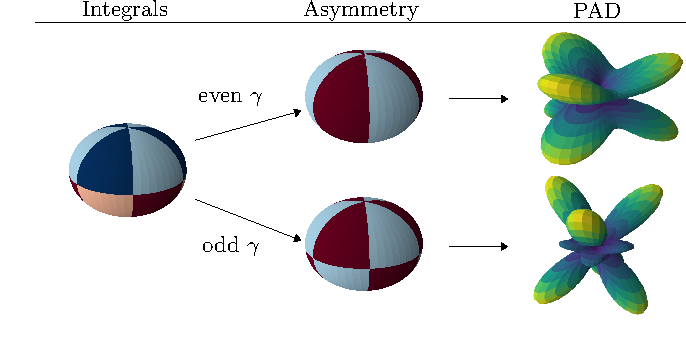
\includegraphics[width=\linewidth]{figs/Photo_ionization/GAP/integral_combined.pdf}
\caption{
Conceptual illustration of GAPs (for $\Delta m=3$). Left: Integrals $I_\pm^{even/odd}$, Eqs.~(3,4), are defined over regions of constructive and destructive inferference, indicated by different colors (dark blue, light blue, dark red, light red), in $xy$-plane.
Middle: GAPs are constructed based on the parity of the parameter $\gamma = l_e+m_e+l_g+m_g+N_p$ from the integrals over the regions denoted by a certain color (light blue, dark red). 
Right: Examplary PADs displaying the asymmetry captured by the parameters for even and odd $\gamma$. (Figure from \cite{venzke2020_GAP})
} 
  \label{fig:integrals}
\end{figure}

To exemplify the significance of the asymmetry parameters we consider the ionization of Ne atom, initially prepared in the $2p_{-1}-3d_2$ superposition (i.e., $\ell_g = 1$, $m_g = -1$, $\ell_e = 2$, $m_e = 2$; and, hence, $l_g + m_g + l_e + m_e = 4$), by an ultrashort intense laser pulse. As discussed at the outset, we expect interferences between two kind of pathways depending on the peak intensity and the pulse duration. 
For an ultrashort pulse at low intensities one-photon transitions from the ground (Fig.\ \ref{fig:scheme_GAP_lin}(c), $N_g = 1$) and the excited states (Fig.\ \ref{fig:scheme_GAP_lin}(a), $N_e = 1$) will interfere, with $N_p = N_g + N_e = 2$, $\gamma = 6$ and $p=0$. An examplary PAD, obtained via numerical TDSE solution in the relevant intensity and pulse duration regimes, is shown at the top of the right column in Fig.~\ref{fig:integrals}. For even $\gamma$ the corresponding parameter $A_0^3$ relates to the difference between the total photoelectron signals in the dark red and light blue shaded regions, as depicted at the top of the middle column of Fig.~\ref{fig:integrals}. Comparison with the PAD shows that this difference indeed accounts for the asymmetry in the PAD induced by the interference of the transition amplitudes for the one-photon processes from the ground and the excited states. In contrast, due to the dependence of multiphoton transition amplitudes on the intensity of the pulse at longer pulse duration and higher intensities it is expected that the one-photon transition from the excited state (Fig. \ref{fig:scheme_GAP_lin}(a), $N_e = 1$) interferes with the two-photon absorption from the ground state (Fig.\ \ref{fig:scheme_GAP_lin}(b), $N_g = 2$), giving rise to $N_p = 3$, $\gamma = 7$ and $p=1$ for ionization of Ne($2p_{-1}-3d_2$). The regions relevant in the calculation of the asymmetry parameter $A_1^3$ and the corresponding exemplary PAD for the Ne atom are presented in the bottom row of Fig.~\ref{fig:integrals}. The comparison indicates the significance of the asymmetry parameter $A_1^3$ for the detection of the interference at high intensities.

\subsubsection{Application via numerical simulations}

For the application of the GAPs we have considered certain superpositions of two atomic states which are first prepared by a pump pulse and then probed by a linearly polarized pulse at a set time delay such that the relative phase between the two states is determined. In the calculations we have therefore simulated the interaction with the probe pulse only by
using numerical solutions of the time-dependent Schr\"odinger equation (TDSE) for the interaction of a electron in a single-active electron (SAE) potential with the electric field $\mathbf{E}$ of a linearly polarized laser pulse (aligned along the quantization ${\hat z}$-axis) in dipole approximation and length gauge with a frequency corrected laser as described in Chapter~\ref{cha:numberic_methods}. The present calculations are performed utilizing single active electron potentials for He atom and Ne atom \cite{reiff2020} with the electron initially prepared in a superposition of the ground and an excited state. The TDSE has been solved by expanding the wavefunction in spherical harmonics (up to $\ell_{max} = 50$ for all relevant $m$ values), as described in Sec.~\ref{sec:short_pulse_effect}. The computations have been performed on a radial grid of 300 a.u.\ with a grid spacing of 0.05 a.u.\, using exterior complex scaling on the outer 15 a.u.\ of the grid. A time step of 0.05 a.u.\ has been used.

\subsection{Results and discussion}

For our applications we have considered individual superposition states in neon (Fig.~\ref{fig:Neon-1-photon}) and realistic superposition states considering all possible initial $m_g$ states of neon and helium atoms (Fig.~\ref{fig:combined_data}). The central frequency of the applied electric field was set to the energy difference of the initially populated field-free states ($\omega_0=|E_g-E_e|$). To analyze the relevance of both the short-pulse parameter $A_0^{\Delta m}$ and the high-intensity parameter $A_1^{\Delta m}$ calculations have been performed for one- and four-cycle probe pulses (FWHM pulse durations) as function of the peak intensity of the pulse. At the end of each simulation of the time-dependent Schr\"odinger equation we obtained the photoelectron angular distribution at a given momentum $k$ (corresponding to a photoelectron energy of $E=2\omega-|E_g|$) by projecting the wavefunction onto the field-free continuum states on the numerical grid. The asymmetry parameters $A_0^{\Delta m}$ and $A_1^{\Delta m}$ are then determined from the numerical PADs using Eq.~(\ref{gaps}).

\begin{figure}[!ht]
\centering
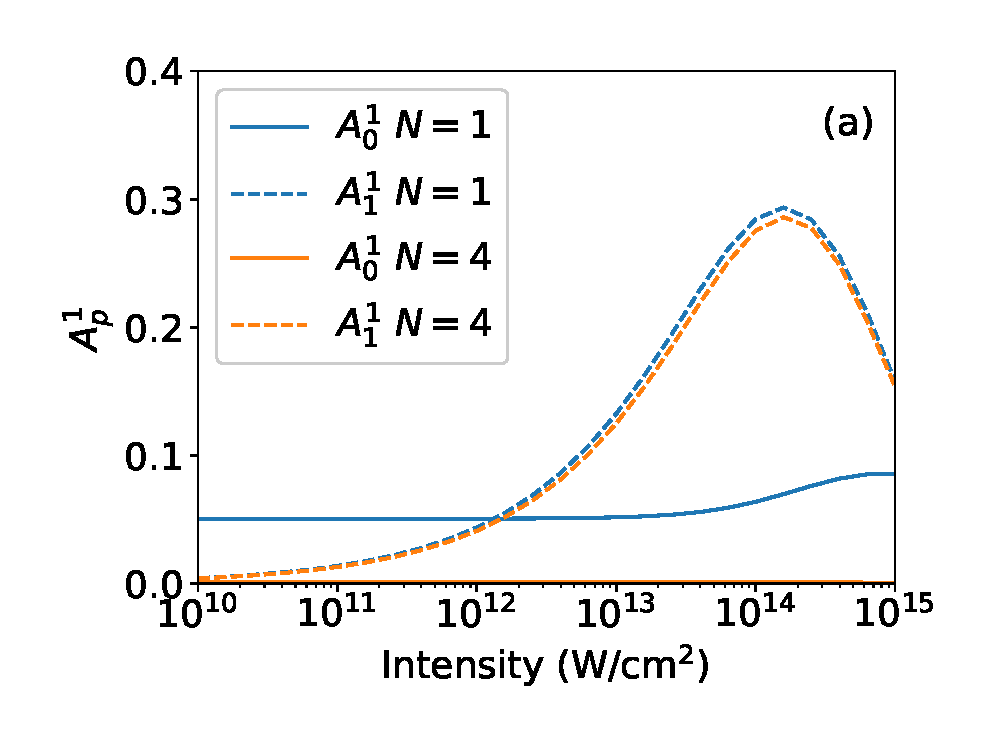
\includegraphics[width=0.32\linewidth]{figs/Photo_ionization/GAP/Ne_2p-1_3d0.eps}
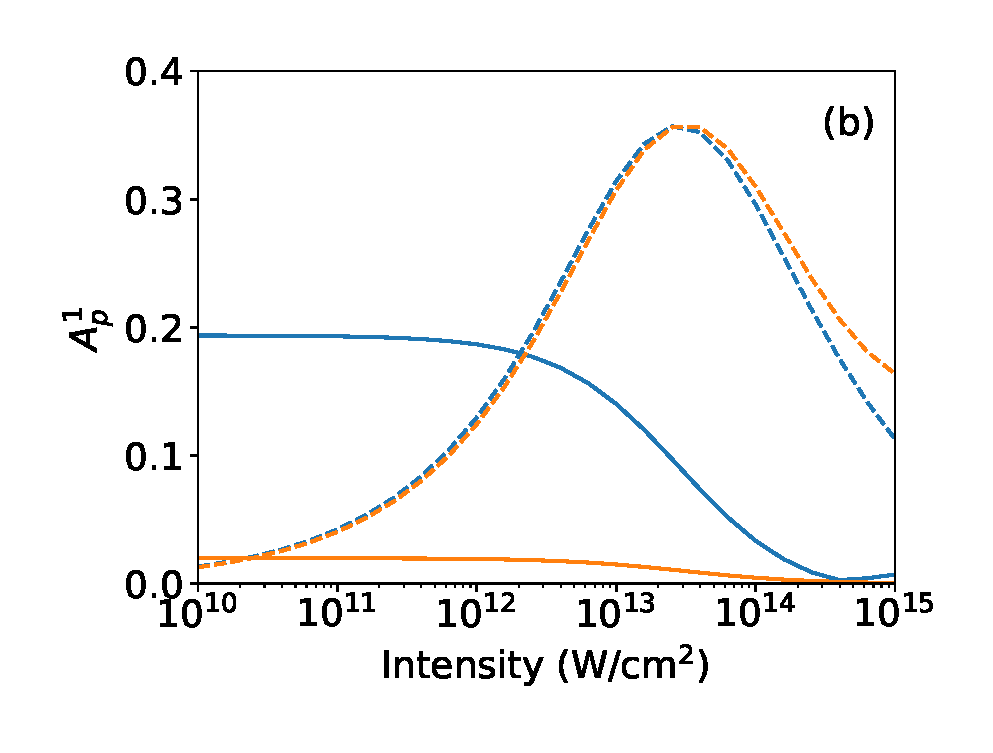
\includegraphics[width=0.32\linewidth]{figs/Photo_ionization/GAP/Ne_2p0_3d1.eps}
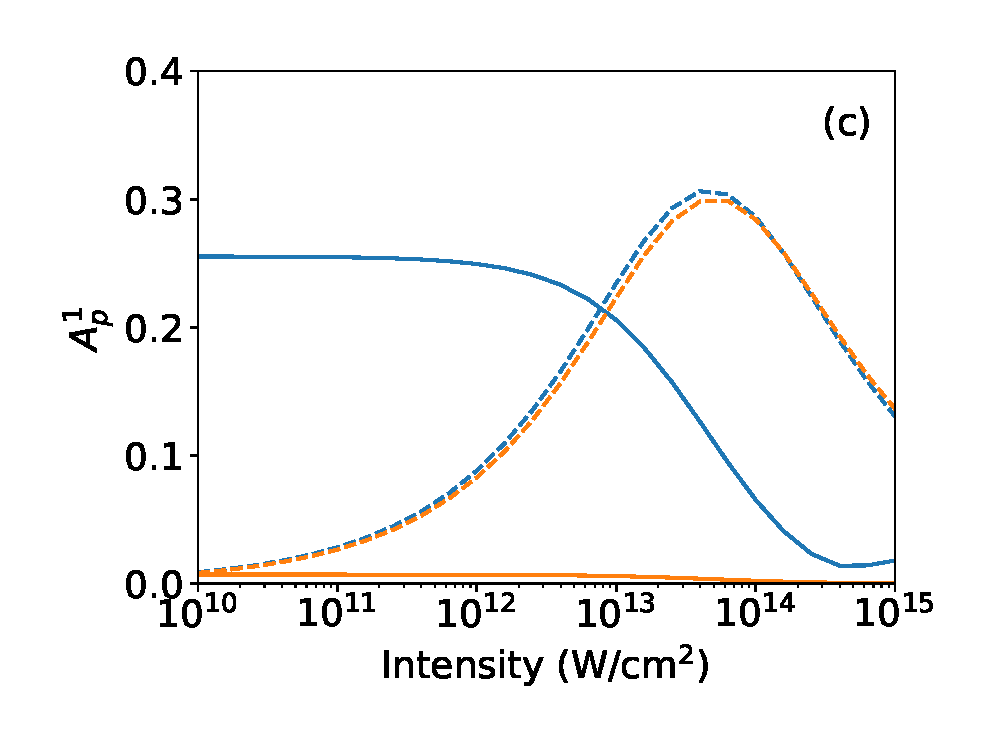
\includegraphics[width=0.32\linewidth]{figs/Photo_ionization/GAP/Ne_2p1_3d2.eps}\\
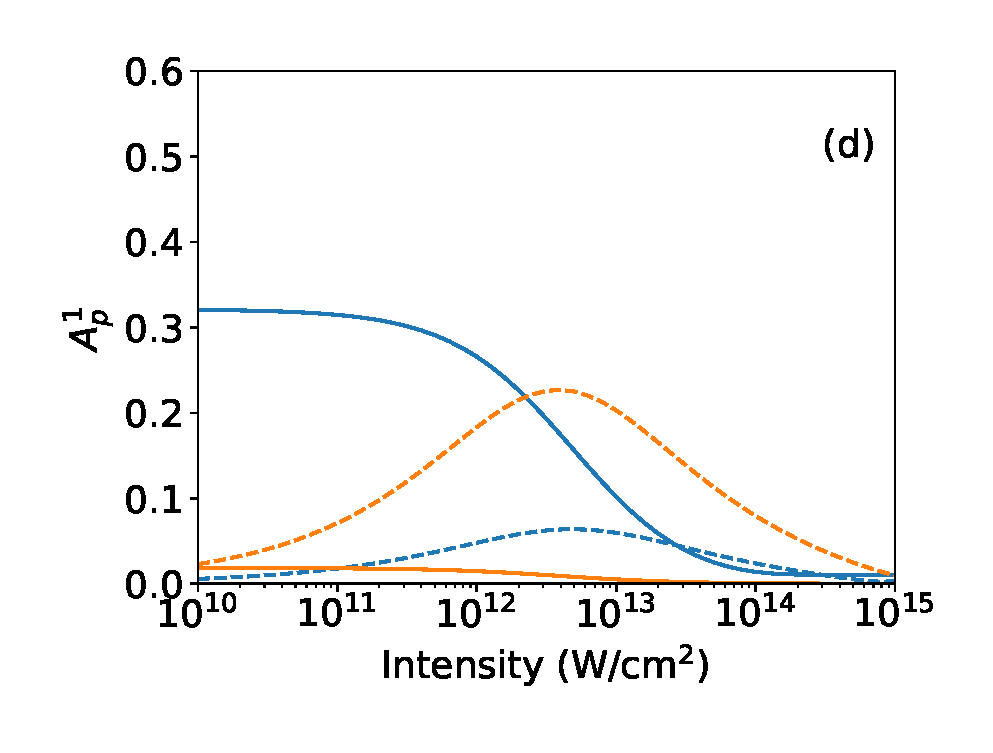
\includegraphics[width=0.32\linewidth]{figs/Photo_ionization/GAP/Ne_2p-1_3d0_real.eps}
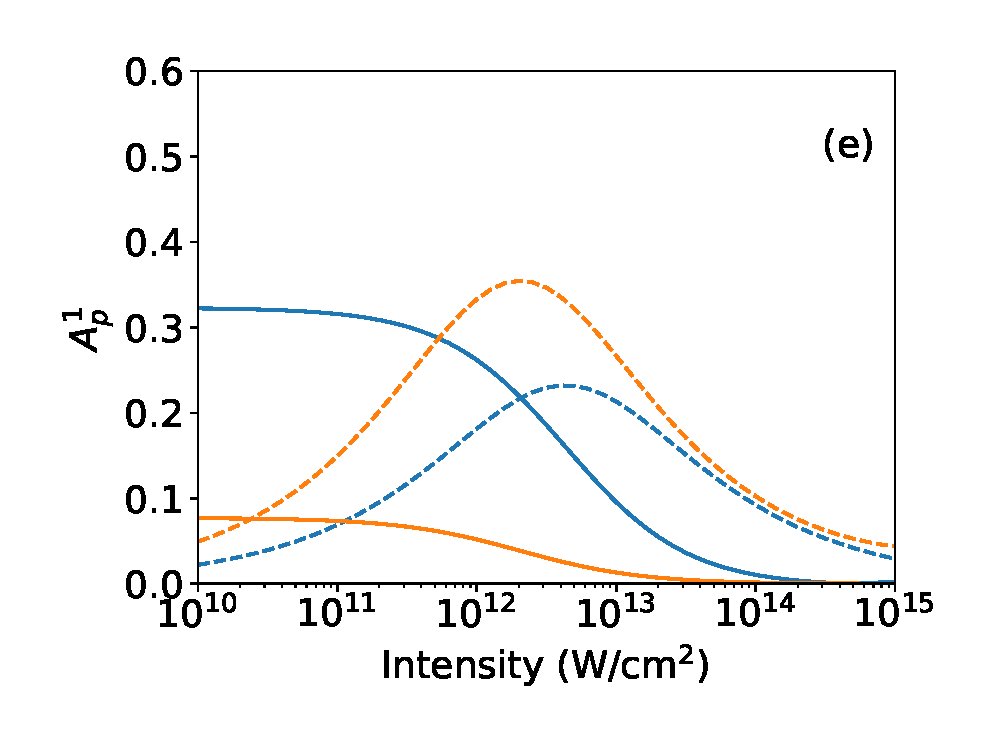
\includegraphics[width=0.32\linewidth]{figs/Photo_ionization/GAP/Ne_2p0_3d1_real.eps}
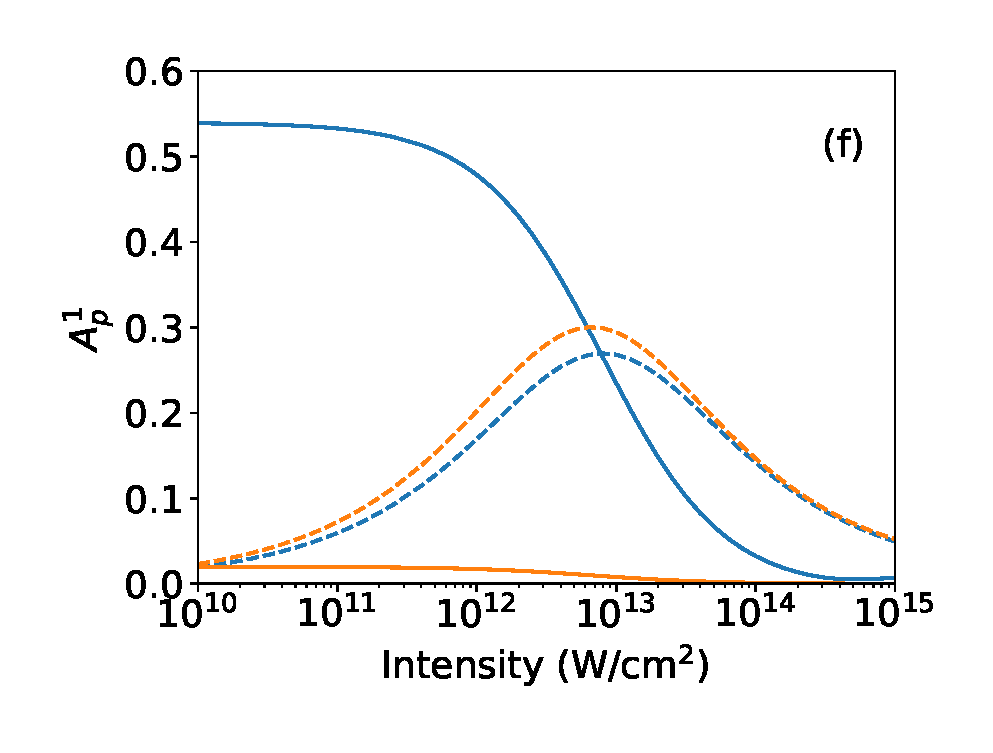
\includegraphics[width=0.32\linewidth]{figs/Photo_ionization/GAP/Ne_2p1_3d2_real.eps}
\caption{
Generalized asymmetry parameters $A_0^1$ (solid lines) and $A_1^1$ (dashed lines) as function of intensity for ionization of  superpositions of $2p_{-1}-3d_0$ (a), $2p_{0}-3d_1$ (b), and $2p_{1}-3d_2$ (c) in neon atom with initial populatations of 0.5 for each state (top row). Results in bottom row for superpositions with populations of $P_{2p_{-1}}=0.98,P_{3d_0}=0.02,P_{4s_0}=0.00057$ (d), $P_{2p_{0}}=0.94,P_{3d_1}=0.06$ (e), and $P_{2p_{1}}=0.88,P_{3d_2}=0.12$ (f). Results have been obtained for one-cycle (blue lines) and four-cycle (orange lines) pulses at photoelectron energy $E = 2\omega-I_p$. (Figure from \cite{venzke2020_GAP})
} 
  \label{fig:Neon-1-photon}
\end{figure}

To exemplify the application and provide basic insights in the relevance of the GAPs, we have first considered superpositions of individual sublevels in different shells of the neon atom as initial state. Fig.~\ref{fig:Neon-1-photon} shows results for the GAPs as a function of peak intensity for interaction of a neon atom, prepared in $(2p_{-1}-3d_0)$ (a,d), $(2p_{0}-3d_1)$ (b,e),  and $(2p_{1}-3d_2)$ (c,f) superpositions. For the results in the top row equal population in the two initial states has been considered, while for those in the bottom row populations, as produced via one-photon excitation by a 50 cycle, $10^{13}$ W/cm$^2$ right handed circulary polarized pump pulse, are used for the initial state  
(states with populations larger than $10^{-5}$ are considered, see figure caption for values). The central frequency of the ionizing probe laser pulse is tuned to the energy gap between the field-free ground and excited states. 

Overall, except for the results in panel (a) which we will discuss below separately, the short-pulse parameter $A_0^1$ (solid lines) is large at low intensities and for the shorter of the two pulse durations. This is expected from our discussion above and confirms that the parameter is an indicator for the interference of the one-photon signal from the ground state and the one-photon signal from the excited state. Since both of these signals
are 
first order in intensity, their relative strengths and, hence, the $A_0^1$ parameter are independent of intensity at low intensities for a given initial superposition state. As the intensity increases, the relative amplitude of the two-photon ionization channel increases and finally dominates over the one-photon channel from the ground state. This trend is reflected in both the short-pulse and the high-intensity parameters. The increase in $A_1^1$, resulting from the interference between the one-photon excited state signal and the two-photon ground state signal, shows in which intensity regime the two-photon signal starts to overtake the short pulse signal. Simultaneously with the increase of $A_1^1$ we observe a decrease of the $A_0^1$ signal, in agreement with our physical interpretation of the relevance of the different pathways. Parenthetically, we note the onset of an increase of the $A_0^1$ parameter at high peak intensities is likely due to pathways involving higher order processes with an even number of total photons.

While the general trends of the two parameters are similar in most of the cases, there is one exception where the details differ significantly. In the case of the $(2p_{-1}-3d_0)/\sqrt{2}$ superposition (panel a), $A_0^1$ shows a different trend. It remains constant at low intensities before increasing at higher intensities. As the laser pulse and relative populations are fixed in the top row (a-c) of Fig.~\ref{fig:Neon-1-photon}, the change in amplitude and shape of $A_0^1$ and $A_1^1$ are caused by changes in the cross-sections of the various states. We, therefore, attribute the different trend in the $A_0^1$ signal in panel (a) to be due to the dominance of the one-photon transition from the $3d_0$ state at all intensities, since $m=0$ states are, in general, easier to ionize with a linearly polarized pulse than those with $|m| > 0$. This interpretation is further supported by the results in Fig.~\ref{fig:Neon-1-photon}(d) for a superposition with much lower initial population in the $3d_0$-state. Despite the difference in magnitude of transition amplitudes, now the interference between the one-photon pathways is effective and the general expected trend for the short-pulse parameter $A_0^1$ is present.

Comparison of the results in the two rows of Fig.~\ref{fig:Neon-1-photon} shows that the intensity at which the transitions in the parameters occur depends on the population in the two states in the initial superposition.
Since in the bottom row the populations in the excited states are low, the relative magnitudes of the corresponding one-photon transition amplitudes from the excited states as compared to those from the ground state levels are weaker than for the equally populated superpositions (top row). Therefore, we observe the impact of the two-photon pathway from the ground state at lower intensities in the results in the bottom row. Additionally, the $A_1^1$ signal becomes sensitive to changes in pulse length due to the weak signal from the excited state. Thus, the GAPs may also be useful to detect the population ratio in the superposition states. Here, we do not further analyze this feature, but focus on the more general application of the parameters to identify the presence of different ionization pathways.

\begin{figure}[!ht]
\centering
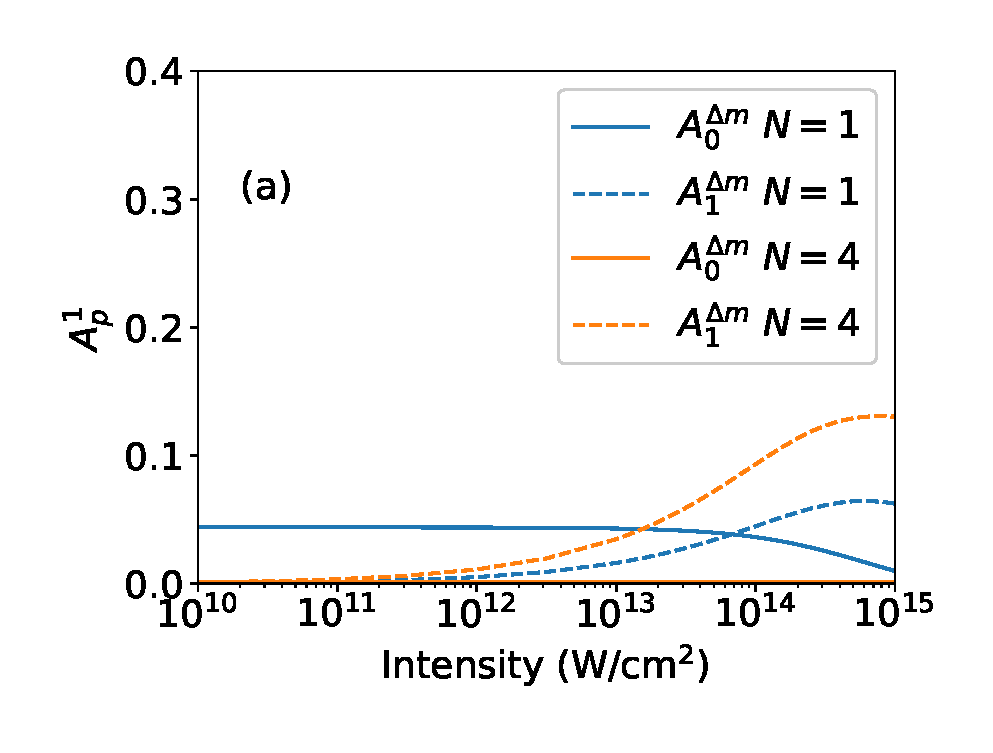
\includegraphics[width=0.32\linewidth]{figs/Photo_ionization/GAP/He_2p1.eps}
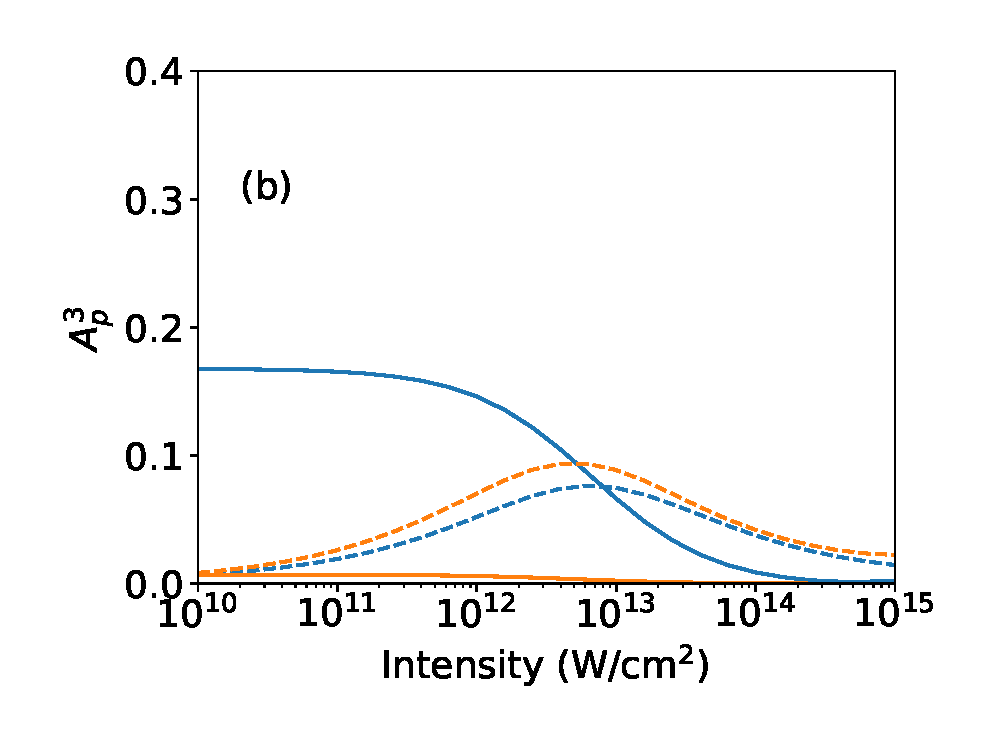
\includegraphics[width=0.32\linewidth]{figs/Photo_ionization/GAP/Ne_2p-1_3d2_3p-combined.eps}
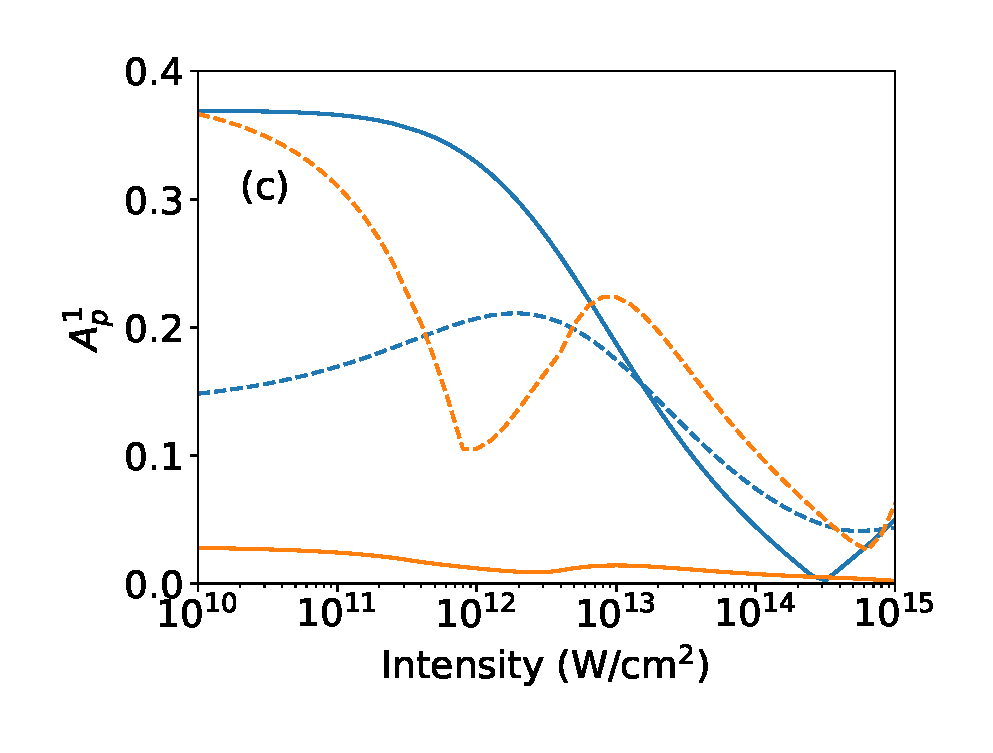
\includegraphics[width=0.32\linewidth]{figs/Photo_ionization/GAP/Ne_2p-1_3d0_1p-combined.eps}
\caption{
Same as Fig.~\ref{fig:Neon-1-photon} but for
superpositions generated by a right-handed circularly polarized pulse
via one-photon transition in helium atom (a),  
three-photon transition in neon atom (b), and 
one-photon transition in neon atom (c) (for details see text). (Figure from \cite{venzke2020_GAP})
} 
  \label{fig:combined_data}
\end{figure}

So far, in Fig.~\ref{fig:Neon-1-photon} we considered simple albeit somehow artificial superposition states restricted to certain sublevels of two shells in the neon atom. Now, we extend our analysis to three different initial states as they can be generated with right-handed circularly polarized pump laser pulses: (a) one-photon excitation of helium atom to the $2p_1$ state leading to $(1s-2p_1)/\sqrt{2}$ superposition, (b) three-photon excitation of neon atom to the $3d$  shell, leading to an initial state consisting of a superposition with equal population in $2p_{-1}$ and $3d_2$ along with populated $2p_0$, and $2p_1$ states (note, that the latter two $2p$ states cannot be excited by the absorption of three right-handed circularly polarized photons to the $3d$ shell), and (c) one-photon excitation of neon atom to the $3d$ shell leading to the combination of the three superposition states analyzed separately in the bottom row of Fig.~\ref{fig:Neon-1-photon}.
In Fig.~\ref{fig:combined_data}, we present results for the GAPs of the corresponding calculations.
The initial superpositions in case of the helium data (a) and the neon data in panel (b) consist of just one state in the excited shell and show the same general trends as those in the majority of the panels of  Fig.~\ref{fig:Neon-1-photon} with the decrease of $A_0^{\Delta m}$ along with the increase of $A_1^{\Delta m}$ occurring in a certain  intensity regime. The transitions in helium occur at a higher peak intensity due to the more tightly bound helium ground state, which is harder to ionize.  
The overall trends of the results in Fig.~\ref{fig:combined_data}(c) for the more complex initial superposition, consisting of six states in the $2p$- and the $3d$-shell of neon.
The one-cycle pulse data are similar to those discussed before, providing the same information about the impact of the two-photon transition from the ground state. However, the $A_1^1$ parameter, particularly at the longer pulse duration, shows an additional interference structure in the transition regime. It is likely that this is due
to an interference between transitions originating from two excited states differing by $\Delta m = 1$, here between one-photon ionization signals
from $3d_0$ and $3d_1$ as well as from $3d_1$ and $3d_2$. Although the number of absorbed photons in these transition is not 3, the resulting $\gamma$ has the same parity as the signal from a $2p_m-3d_{m+1}$ state.

\begin{figure}[!ht]
\centering
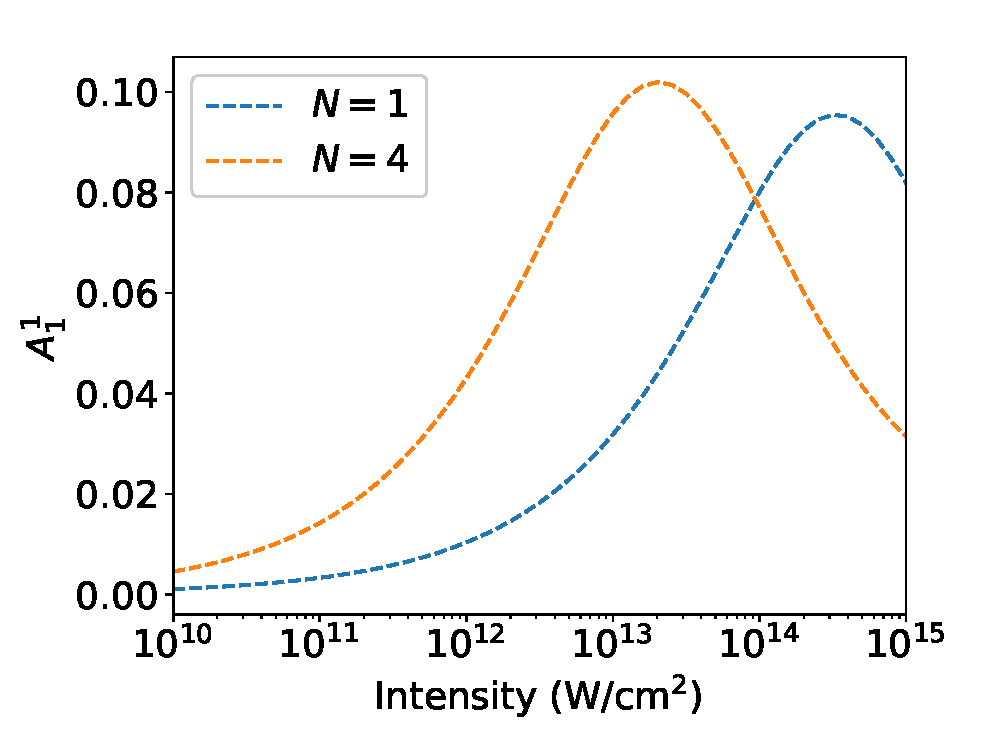
\includegraphics[width=.45\linewidth]{figs/Photo_ionization/GAP/He_2p1_detune_1p2.eps}
\caption{ 
Asymmetry parameter $A_1^1$ for ionization of helium atom ($1s$-$2p_1$) with one- and four-cycle pulses at central frequency 
$\omega=1.2\omega_0$. (Figure from \cite{venzke2020_GAP})
} 
  \label{fig:detuned_GAP}
\end{figure}

The high-intensity asymmetry parameter $A_1^{\Delta m}$ is not only indicative of the general features concerning the interferences between the pathways discussed above, but also provides insights in more subtle aspects. In the top row of Fig.~\ref{fig:Neon-1-photon} the maximum of the asymmetry parameter $A_1^{\Delta m}$ occurs at the same intensity independent of the pulse duration. This is due to the fact that in the calculations the central frequency was set to the energy difference of the initially populated states. In this case the center of the photoelectron energy distributions due to the one-photon ionization from the excited state and the two-photon transition from the ground state nearly coincide. If the frequency is detuned from the resonance, the position of maximum interference strongly depends on the pulse duration. Due to the larger spectral width of the pulse at shorter pulse duration, the interference between the channels becomes most effective at higher intensities than the longer pulse duration results, at which the photoelectron distributions from the two channels have less overlap. This effect is seen in the results in Fig.\ \ref{fig:detuned_GAP} for photoionization at a central frequency of 1.2 times the energy difference between the $1s$- and $2p_1$-states in helium atom. 

\begin{figure}[!ht]
\centering
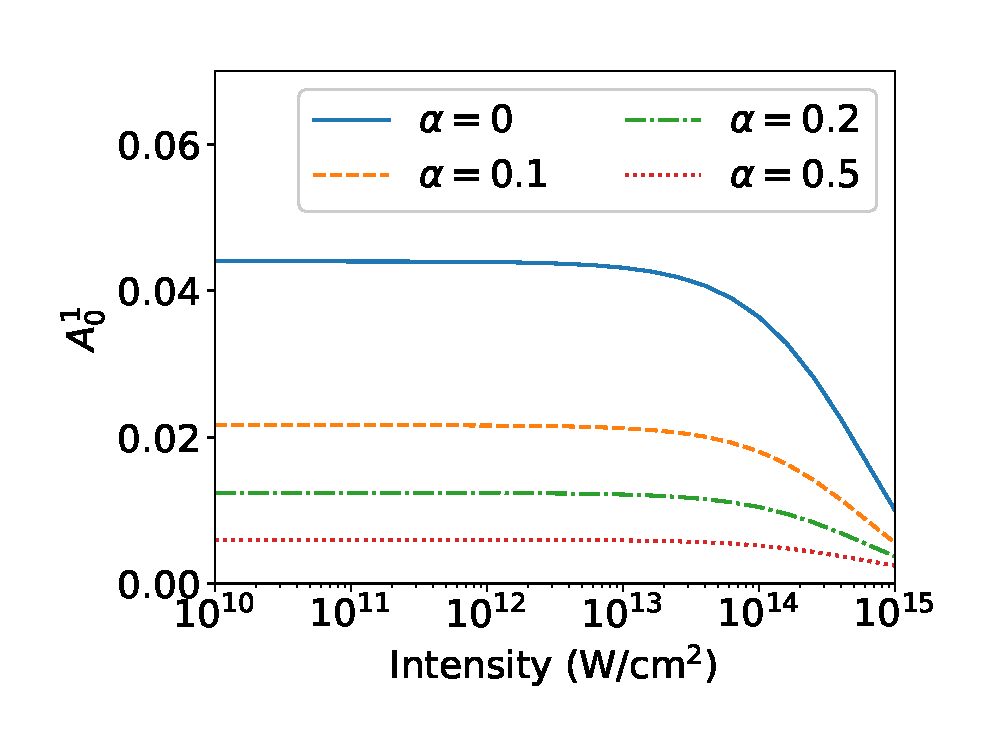
\includegraphics[width=.45\linewidth]{figs/Photo_ionization/GAP/He_2p1_asym_alpha.eps}
\caption{
Asymmetry parameter $A_0^1$ for ionization of helium atom ($1s$-$2p_1$) with one-cycle pulses at central frequency $\omega_0$. Results of averages over different Gaussian distributions of CEP with width $\alpha$ are compared with those at fixed CEP ($\alpha =0$, solid line). (Figure from \cite{venzke2020_GAP})
} 
  \label{fig:cep_avg}
\end{figure}

Finally, it is important to consider variations in the laser parameters relevant for an application of the generalized asymmetry parameters in an experiment. Typically, the peak intensity of the applied laser pulse may vary from shot to shot as well as over the interaction volume. The results in Fig.\ \ref{fig:Neon-1-photon} and Fig.\ \ref{fig:combined_data} show that the two GAPs vary rather slowly as a function of peak intensity. Thus, we can expect that variations in intensity in an experiment will not impact the results significantly. Another parameter that is usually difficult to control is the CEP of a laser pulse, which typically becomes most important for ultrashort pulses. In the present study the high-intensity $A_1^{1}$ parameter is independent of variations in CEP. To study the dependence on the CEP for the short-pulse low-intensity asymmetry parameter $A_0^{1}$ we have obtained results as a function of the CEP and averaged the results about a given value $\varphi_0$ using a Gaussian distribution of width $\alpha$ (in units of $2\pi$) as: 
%
\begin{equation}
A_{p}^{\Delta m}(I, T; \alpha)
= 
\frac{\sum_i \exp\left[-\frac{1}{2}\left(\frac{|\varphi_i-\varphi_0|}{2\pi\alpha}\right)\right] \sigma(\varphi_i) A_{p}^{\Delta m}(\varphi_i,I,T) }
{\sum_i\exp\left[-\frac{1}{2}\left(\frac{|\varphi_i-\varphi_0|}{2\pi\alpha}\right)\right]\sigma(\varphi_i)}\; ,
    \label{eq:PAD_gauss_window}
\end{equation}
%
where $\sigma(\varphi_i)$ is the total ionization probability at CEP $\varphi_i$. 
In the calculations we have assumed that the pump pulse (for the preparation of the initial state) has the same CEP as the probe pulse.
The comparison of the results for different averages in Fig.\ \ref{fig:cep_avg} with the results for fixed CEP (solid line) shows that for He atom the short-pulse asymmetry parameter $A_0^1$ is indicative for the interference up to fluctuations of about $\pi/2$ in the CEP. 


\subsection{Summary}

%The Discussion should be succinct and must not contain subheadings.

In summary, in this section we have introduced a set of generalized asymmetry parameters (GAPs) which characterize the interference of linear and nonlinear pathways to ionization of atoms, prepared in superposition states, due to the interaction with a linearly polarized intense ultrashort laser pulse. These parameters may provide a new tool to analyze data in attosecond experiments. The relevance of the parameters is demonstrated via the results of numerical simulations of ionization of helium and neon atom. The impact of short pulse and nonlinear effects, as they arise in experiments with free-electron lasers and high-order harmonic generation, is shown. The dependence on the central frequency of the applied laser pulse and the impact of variations of laser parameters, such as the peak intensity and the carrier-to-envelope phase, are analyzed and discussed.

%%%%%%%%%%%%%%%%%%%%%%%%%%%%%%%%%%%%%%%%%%%%%%%%%%%%%%%%%%%%%%%%%%%%%%%%%%%%%%%%%%%%%%%%%%%%%%%%%%%%%%%%%%%%%%%%%%
%%%%%%%%%%%%%%%%%%%%%%%%%%%%%%%%%%%%%%%%%%%%%%%%%%%%%%%%%%%%%%%%%%%%%%%%%%%%%%%%%%%%%%%%%%%%%%%%%%%%%%%%%%%%%%%%%%
%%%%%%%%%%%%%%%%%%%%%%%%%%%%%%%%%%%%%%%%%%%%%%%%%%%%%%%%%%%%%%%%%%%%%%%%%%%%%%%%%%%%%%%%%%%%%%%%%%%%%%%%%%%%%%%%%%
%%%%%%%%%%%%%%%%%%%%%%%%%%%%%%%%%%%%%%%%%%%%%%%%%%%%%%%%%%%%%%%%%%%%%%%%%%%%%%%%%%%%%%%%%%%%%%%%%%%%%%%%%%%%%%%%%%
%%%%%%%%%%%%%%%%%%%%%%%%%%%%%%%%%%%%%%%%%%%%%%%%%%%%%%%%%%%%%%%%%%%%%%%%%%%%%%%%%%%%%%%%%%%%%%%%%%%%%%%%%%%%%%%%%%
\section[Wavefunction reconstruction method]{Wavefunction reconstruction method\protect\footnote{The content of this section has been also published in J. Venzke et al., PRA. \textbf{103}, 042808 (2021).}} % (fold)
\label{sec:wavefunction_reconstruction}
% The availability of ultrafast light sources at wavelengths from the vacuum ultraviolet (VUV) and extreme ultraviolet (EUV) to the soft X-ray regime via the technologies of free electron lasers (FEL) \cite{seddon2017} and high-order harmonic generation (HHG) \cite{popmintchev2010,chini2014} has opened a new regime of ultrafast measurements in atomic and molecular physics. Laser pulses of duration as short as a few tens of attoseconds have been demonstrated experimentally \cite{zhao2012,chen2014} and enabled the observation of electron dynamics (for recent reviews, see \cite{vrakking2014,pazourek2015,calegari2016,ramasesha2016,young2018,peng2019}). One example is the time-resolved measurement of the photoelectric effect in atoms and solids \cite{cavalieri2007,schultze2010,klunder2011,tao2016,isinger2017}. Electron emission from the target has been also temporally resolved for a transition of the electron into the continuum through excited state resonances \cite{su2015,Sabbar2015,Gong2017}, autoionizing states \cite{jimenez2014,Dolmatov2015,Barreau2019}, Fano resonances \cite{kaldun2016,kotur2016,gruson2016,cirelli2018} and for correlated electron emission \cite{pfeiffer2011,pazourek2012,mansson2014}. Electron wave packet dynamics in superposition states of atoms and molecules has been another focus of ultrafast time-resolved studies, either for single valence electron motion \cite{goulielmakis2010,mauritsson2010,holler2011,hockett2011,Kim2012,xie2012,klunder2013,beck2014,hassan2016,walt2017,priebe2017,He2018} or correlated two-electron dynamics \cite{hu2006,feist2011,ott2014}.

% Recently, the application range of ultrafast laser pulse technology has been extended by the capability to control the polarization of the emitted light in high-order harmonic generation and free electron lasers. The physical principle to produce circularly polarized high-order harmonics has been proposed and applied first two decades ago \cite{eichmann1995}. Efficient phase matching of the generated light in the EUV and soft X-ray regime \cite{fleischer2014,fan2015,hickstein2015} and the control of the polarization stage \cite{huang2018} has been demonstrated more recently. Similarly, free electron laser light with variable polarization has become available \cite{spezzani2011,mazza2014}. The potential to control the polarization and helicity of light generated by HHG and FELs extends the range of accessible states and transition pathways during photon absorption. States with varying orbital angular momentum and magnetic quantum number can be excited during the interaction with the pulses. In turn, the helicity of the light pulses can be used to selectively prepare superpositions of states in atoms or molecules with a variety of combinations in the quantum numbers (principal, orbital angular momentum, magnetic) on an ultrafast time scale. 

As mentioned above, one of the simplest cases of a superposition of atomic states with different orbital angular momentum and magnetic quantum numbers is that of a helium atom in the $1s$ and $2p_1$ states. It results in an ultrafast electron dynamics given by a wave packet rotating in a plane around the nucleus with a period of $\sim200$ attoseconds. We now use this dynamics as a prototype example to study the reconstruction of the corresponding wave packet via ionization with an ultrashort linearly polarized probe laser pulse.  To this end, we analyze the photoelectron angular distributions as a function of time delay from the instant of preparation of the atomic superposition states. The concept is based on the idea to utilize quantum beating signals, where the imaged wave packet is interfered with a reference wave, to reconstruct a wave function \cite{paul2001,muller2002,mauritsson2010,klunder2013,priebe2017,jiang2020}. Accounting for the phase accumulation, ionization cross sections, and characterization of the reference wave packet that is used in the measurement is a non-trivial task. In this section we present a method for wave packet reconstruction based on quantum beating signals that utilizes perturbation theory. Since the method requires knowledge of the average values for intensity, carrier-to-envelope phase and pulse duration of the probe pulse we perform a sensitivity study to show the impacts of noise produced in an experiment and the limits in peak laser intensity on the reconstruction method. Finally, we consider the extension of the method to  imaging of wave packets consisting of superpositions of more than two states.

The rest of the section is organized as follows: In section \ref{sub:theory} we first present and discuss the ionization scheme on which the reconstruction method is based. Then we briefly review the methods for the numerical methods used for the reconstruction algorithm. In section \ref{sub:results} we present the application of the method to the reconstruction of a circular wave packet in helium atom. Aspects of the error analysis with respect to the accuracy of the observation of the PADs and the variation of the laser parameters will be presented. Furthermore, the impact of different pathways on the reconstruction process will be studied. Finally, we briefly discuss the extension of the method to superpositions of more than two states along with results for a specific three-state superposition. The section ends with a summary. 

\subsection{\label{sub:theory}Concept and theoretical methods}
%%%%%%%%%%%%%%%%%%%%%%%%%%%%%%%%%%%%%%%%%%%%%%%%%%

\subsubsection{Pump-probe scheme}
%%%%%%%%%%%%%%%%%%%%%%%%%%%%%%

In this study, we focus on the reconstruction of a wave function and the related imaging of the dynamics via photoelectron angular distributions (PAD). To this end, we start our simulations in a superposition state of the atom. An experiment will require a pump pulse to generate the superposition. There are a few requirements for the pump pulse itself to apply the reconstruction scheme. Since the scheme relies on the measurement of the PADs at various time delays between the pump and the probe pulse, the pump must be a reproducible pulse with a fixed carrier envelope phase (CEP) such that the superposition generated for each measurement is very similar from shot to shot if not the same. However, the form of the electric field of the pump pulse does not need to be known. Next, the delay between the pump and probe pulses must be controlled on the attosecond time scale to allow for measurements as a function of the delay. The shot-to-shot measurements should be taken for time delays within one cycle of the probe pulse giving rise to the requirement of an attosecond control over the delay. The total delay is irrelevant as long as the two pulses do not overlap in time and the state to be imaged does not decay. Furthermore,
photoelectrons generated by the pump pulse have to be separated from those produced by the probe pulse. It might be therefore useful to limit ionization by the pump pulse.

\begin{figure}[!ht]
\centering
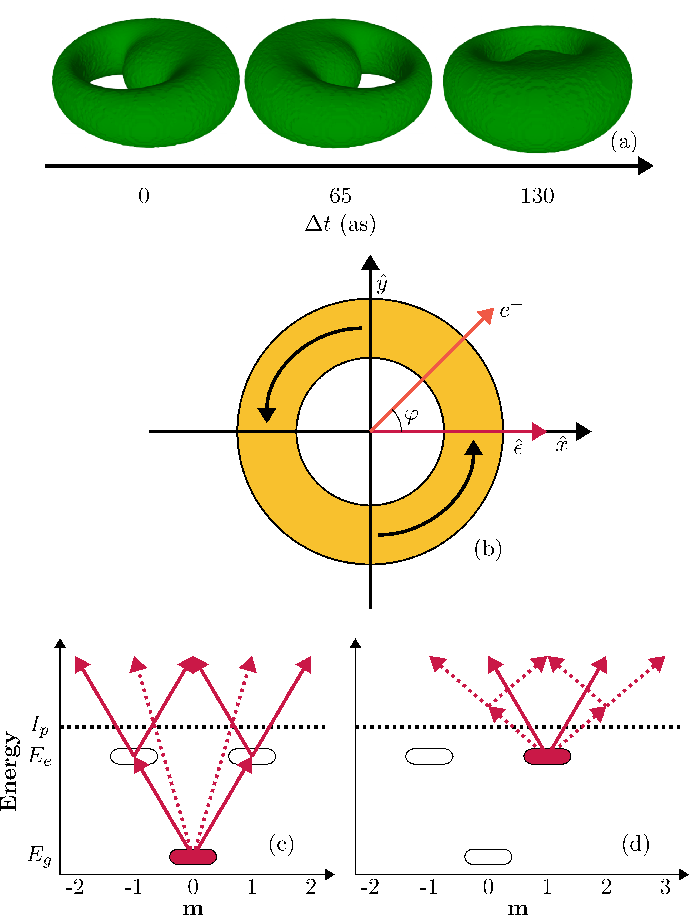
\includegraphics[width=0.7\linewidth]{figs/Photo_ionization/superpositions/Venzke_new_fig_1.eps}
\caption{(a) Isosurfaces of the $1s-2p_1$ wave function ($|r\Psi|^2$ is shown) evolving in time. (b) Ionization scheme in the $x-y$ plane. The laser polarization along the $x$-axis is depicted in red, the direction of the ionized electron is shown in orange, and the charge migration is shown in yellow. Selection rules for ground state signal (c) and excited state signal (d). The solid lines illustrate the transitions of photons absorbed at the central frequency and the dashed lines show the pathways for short pulse effect due to the large bandwidth of an ultrashort pulse. (Figure from \cite{venzke2021_wave})
} 
  \label{fig:dynamic_visualization}
\end{figure}

The method studied here can be applied to simple superpositions, consisting of population in two or three atomic states. As prototypical example we consider a helium atom in a $1s-2p_1$ superposition, which represents a circular wave packet rotating around the nucleus. This superposition with equal population in the two levels can be created with a $\sim23$ cycle laser pulse at $10^{14}$ W/cm$^2$ tuned to the resonance frequency. Fig.~\ref{fig:dynamic_visualization}(a) shows the dynamics via isosurfaces of the wave function (i.e., $\left|r\Psi\right|^2$) rotating in the $x-y$ plane on an attosecond time scale. 

To characterize the motion, and in turn reconstruct the wave function, we expand the initial wave function in the eigenbasis of stationary states and write the wave function at some time $t$ as: 
%
\begin{equation}
    \Psi({\bm r},t) = a_0 \psi_0({\bm r},t) + \sum_{j=1}^{N-1} a_j e^{i\theta_j} \psi_j({\bm r},t)
    \label{eq:expansion}
\end{equation}
%
where $a_j$ is a positive real number, $\theta_j $ is a relative phase, and $\{ \psi_j = \Psi_{nlm}; j = 0, \ldots, N-1\}$ is the eigenstate basis. While the basis may contain an infinite number of eigenstates, for practical means in the numerical calculations and any application it has to be truncated at some finite number $N$. Thus, the wave function depends on $N-1$ phases and $N$ amplitudes since the global phase is not a physically relevant quantity. In this framework, the time dependence is contained in the states $\ket{\psi_j(t)}$ and the initial wave function is completely reconstructed if all $a_j$ and $\theta_j$ for $j\geq 1$ are obtained since $a_0$ is fixed by the normalization and we set the phase of ground state $\ket{\psi_0}$ to zero. If the wave function generated by the pump pulse can be reconstructed at a given time, the full time dependent motion of the wave function has also been obtained.

In the reconstruction scheme that we consider the electron dynamics is probed via ionization by an intense ultrashort laser pulse as a function of time delay  after the end of the pump pulse. In the scheme predictions of first- and second-order perturbation theory (PT) are used to determine the unknown phases and amplitudes from the photoelectron angular distributions (PADs). The latter may be determined in an experiment but in this theoretical study we utilize ab-initio numerical calculations. For the case of a helium atom in a $1s-2p_1$ superposition, we apply a probe laser pulse linearly polarized along the $x$-axis and detect the photoelectron angular distribution in the $x-y$ plane, i.e.\ for $\theta = \pi/2$, as a function of the angle $\varphi$ from the $x$-axis as shown in Fig.~\ref{fig:dynamic_visualization}(b). The absorption of a photon will induce transitions with $\ell \rightarrow \ell \pm 1$ and $m \rightarrow m \pm 1$ due to the selection rules. The pathways from the ground (c) and the excited state (d) are shown in Fig.\ \ref{fig:dynamic_visualization}. The solid arrows represent the pathways for the transitions at the central frequency of the probe pulse. $I_p$ is the ionization potential and the ovals indicate possible resonances. Since we analyze photolelectron emission induced by ultrashort pulses, we need to consider additional pathways due to the broad bandwidth of the pulse (Sec.~\ref{sec:short_pulse_effect}). These pathways are the ionization from the ground state with a single photon and the two-photon transition from the excited state, which are represented by the dotted arrows in Fig.~\ref{fig:dynamic_visualization}. Since states in the continuum with the same energy and quantum numbers can be reached via different pathways, the photoelectron angular distribution will change in both shape and yield as the relative amplitudes and phases of each signal varies.

\subsubsection{Numerical solution of time-dependent Schr\"odinger equation}
%%%%%%%%%%%%%%%%%%%%%%%%%%%%%%%%%%%%%%%%%%%%%%%%

In order to test the applicability and limits of the reconstruction method we use numerical solutions of the time-dependent Schr\"odinger equation (TDSE) as substitute for actual measurements of the photoelectron angular distributions. We consider the TDSE in length gauge and single-active electron approximation as described in Chapter~\ref{cha:numberic_methods}. We use a Helium SAE potential
giving a ground state energy of -0.944409 a.u. and a $2p$ energy of -0.12847 a.u. The potential has been constructed for benchmark tests between TDSE and time-dependent density functional theory (TDDFT) calculations \cite{reiff2020}. The energies match those of the corresponding DFT potential while the experimental values for the ground and the $2p$ state in helium are -0.9037 a.u. and -0.12382 a.u.

For the solution we have expanded $\Psi(\mathbf{r},t)$ in spherical harmonics up to $l_{max} = |m_{max}| = 20$ and discretized the radius using fourth order finite difference. The wave function has been propagated in time with a time step of 0.01 a.u., on a grid with spacing of 0.05 a.u., maximum radius of 300 a.u., and exterior complex scaling on the outer 30 a.u. of the grid utilizing the Crank-Nicolson method for time propagation. The numerical code has been tested against previously used codes as well as results from numerical calculations published in the literature \cite{Scrinzi2010}. The electric field is a frequency corrected sine squared pulse.
Once the wave function has been propagated to the end of the pulse we have obtained the photoelectron angular distribution  by projecting onto numerical continuum states. 

\subsubsection{Perturbation theory}
%%%%%%%%%%%%%%%%%%%%%%%%%%%%%%%%

To reconstruct the initial wave function, i.e. determine amplitudes and phases, we invert the photoelectron angular distributions (here, TDSE results) as a function of time delay by utilizing perturbation theory (PT) described in Sec.~\ref{sec:perturbation_theory}. To evaluate the PT wavefunction, we use the bound states of the TDSE field free Hamiltonian for the initial states, and expand the Green's function for 200 dipole allowed states per $\ell$ and $m$ block. The states represent the bound part of the spectrum and a discretized continuum up to an energy of $\sim59$ eV.
The matrix elements and time integrals are performed numerically.

The PT results are then used to obtain a residual 
%
\begin{align}
   R(\mathbf{a}) &=
   \sum_{k,\phi,\tau} \left|\frac{P_\text{TDSE}}{\sum\limits_{k,\phi,\tau}|P_\text{TDSE}|}-\frac{P_\text{PT}(\mathbf{a})}{\sum\limits_{k,\phi,\tau}|P_\text{PT}(\mathbf{a})|}\right|^2
   \label{eqn:residual}
\end{align}
%
where $P_\text{TDSE}$ and $P_\text{PT}$ are the TDSE and PT photoelectron distributions for all utilized final momenta, time delays, and detection angles. The state vector $\mathbf{a}$ that minimizes $R(\mathbf{a})$ gives the reconstructed wave function. The normalization maintains the relative yields at each final momentum. To minimize $R(\mathbf{a})$ for the two (three) state system considered below, 1000 (250) evenly spaced samples were used. 
For the current applications, this minimization technique is sufficient. For superpositions involving more states the dimensionality of the minimization space increases. It is likely that for such studies more advanced minimization methods such as stochastic gradient descent will be needed. We also note that the method is applied to image field-free wave packets, i.e. $\mathbf{a}$ is time independent. For cases, in which $\mathbf{a}$ changes with time, an extension of the present method is needed.

\subsection{\label{sub:results}Results and discussion}
%%%%%%%%%%%%%%%%%%%%%%%%%%%%%%%%

\subsubsection{Reconstruction of two-state superposition: Intensity limits and number of samples}
%%%%%%%%%%%

\begin{figure}[!ht]
\centering
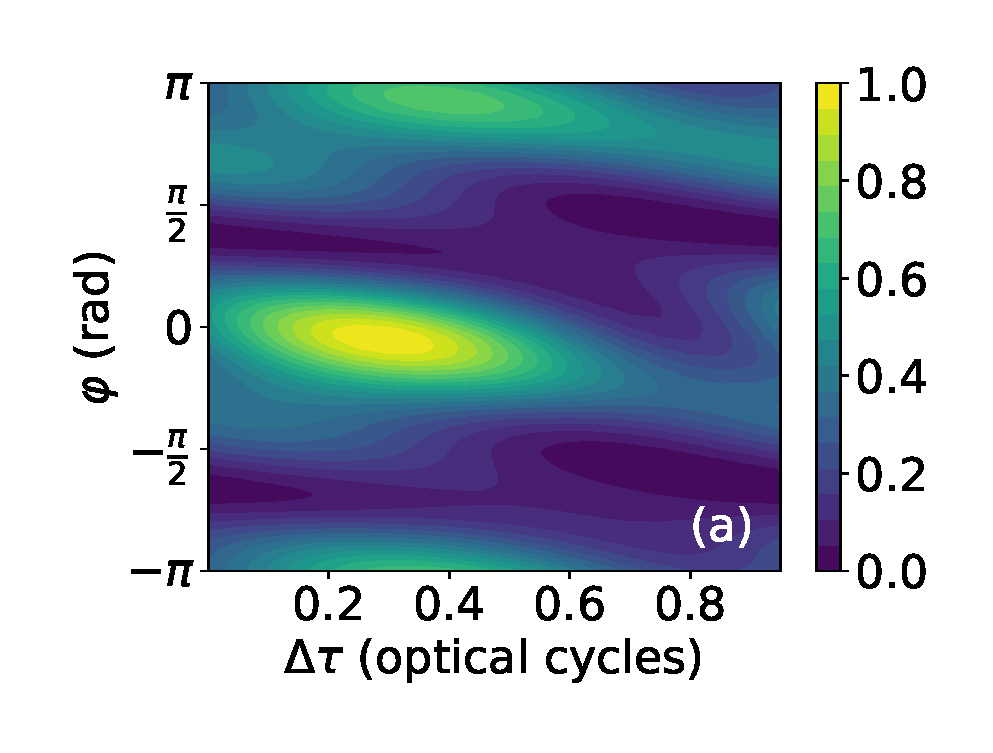
\includegraphics[width=0.4\linewidth]{figs/Photo_ionization/superpositions/Venzke_new_fig_2a.eps}
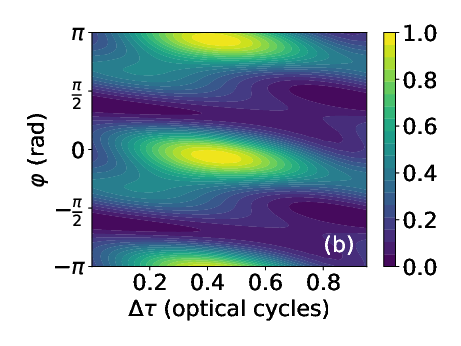
\includegraphics[width=0.4\linewidth]{figs/Photo_ionization/superpositions/Venzke_new_fig_2b.eps}\\
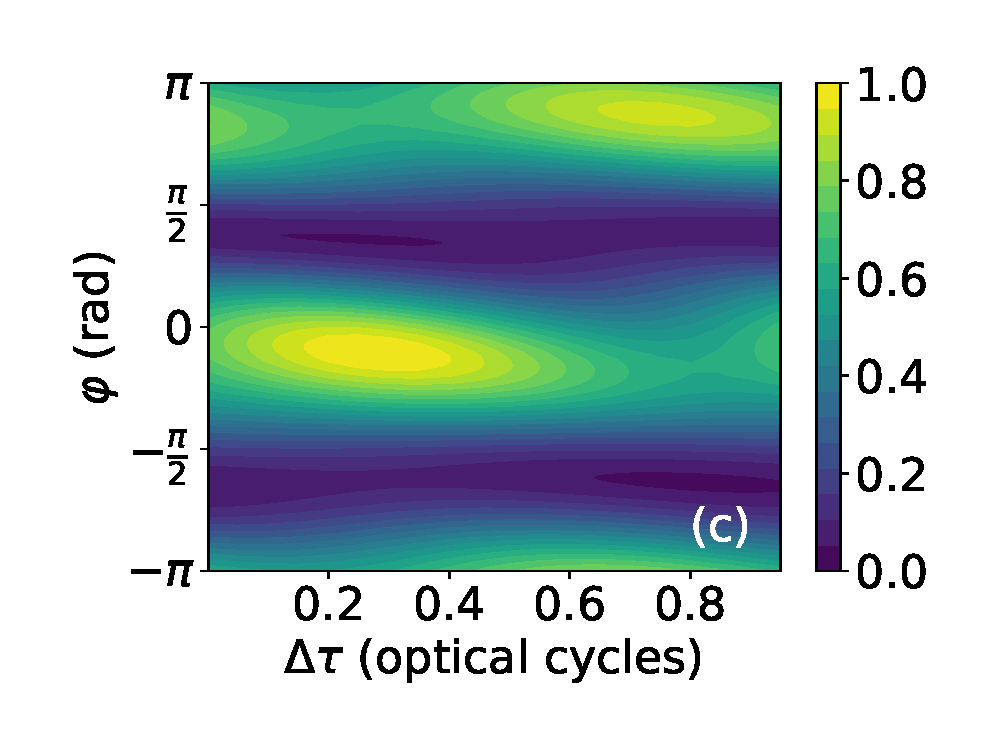
\includegraphics[width=0.4\linewidth]{figs/Photo_ionization/superpositions/Venzke_new_fig_2c.eps}
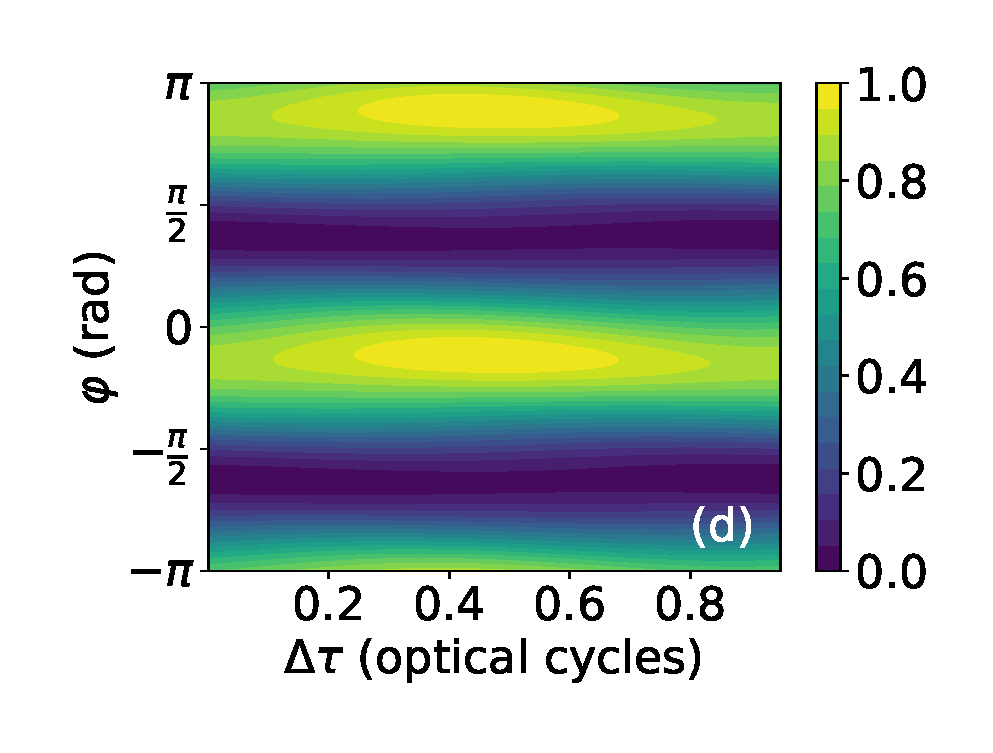
\includegraphics[width=0.4\linewidth]{figs/Photo_ionization/superpositions/Venzke_new_fig_2d.eps}\\
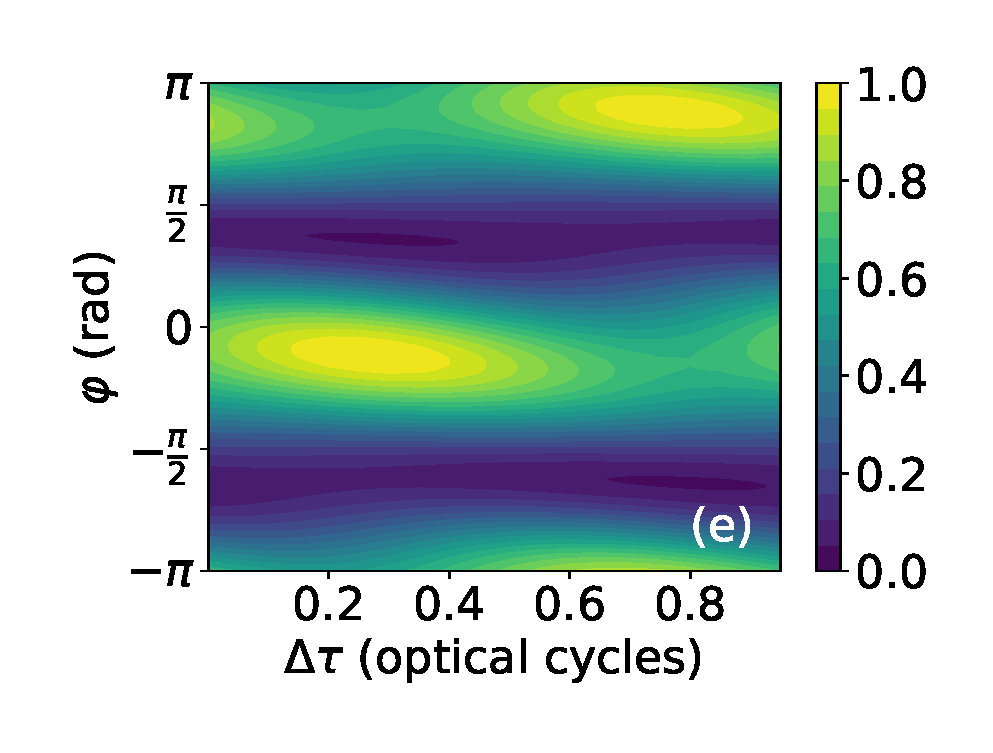
\includegraphics[width=0.4\linewidth]{figs/Photo_ionization/superpositions/Venzke_new_fig_2e.eps}
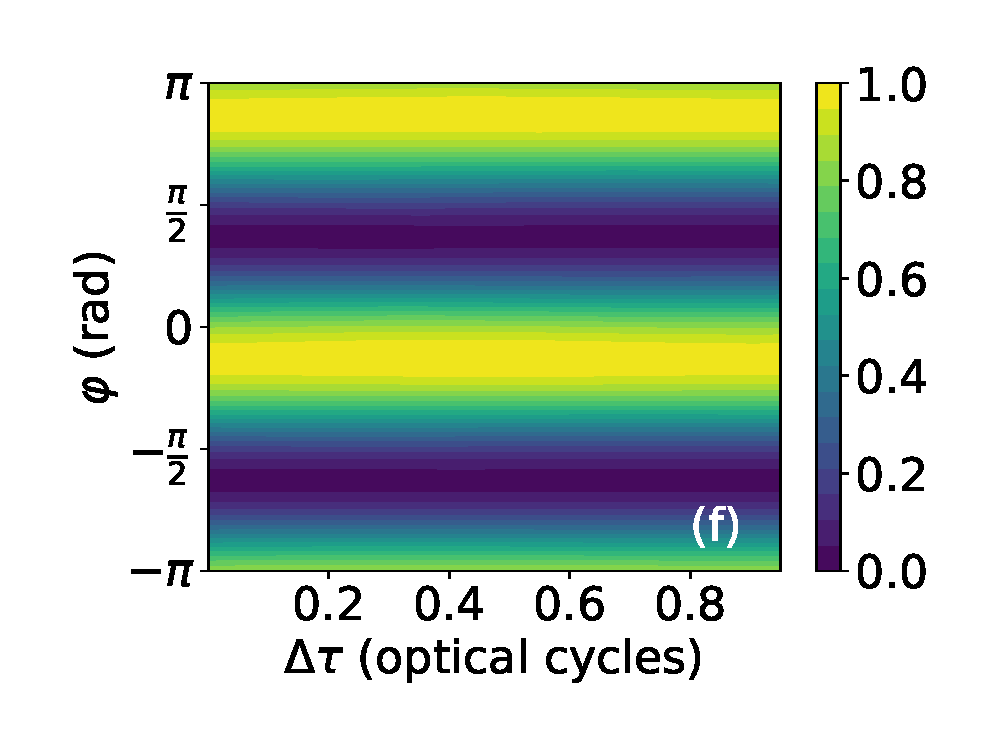
\includegraphics[width=0.4\linewidth]{figs/Photo_ionization/superpositions/Venzke_new_fig_2f.eps}\\
\caption{
Results of TDSE calculations for photoelectron angular distributions over one cycle of the probe pulse field for ionization of $1s - 2p_1$ superposition with ultrashort two-cycle (left column) and ten-cycle (right column) laser pulse with peak intensities of $10^{14}$ W/cm$^2$ (top row), $10^{12}$ W/cm$^2$ (middle row), and $10^{10}$ W/cm$^2$ (bottom row). The time delays $\Delta \tau$ are given with respect to a reference time $\tau_0$ after the end of the first pulse. (Figure from \cite{venzke2021_wave})
} 
  \label{fig:pad_vs_time}
\end{figure}

To apply the minimization and therefore reconstruct the wave packet, the photoelectron angular distributions (PADs) have to vary as a function of time delay. It is therefore first interesting to see at which laser parameters a significant variation in the PADs can be observed. To this end,
in Fig.~\ref{fig:pad_vs_time} we show how the PAD varies within one optical cycle of the pump pulse.
The delay $\Delta \tau$ in the Figure refers to some fixed reference time $\tau_0$ after the end of the first pulse. Comparison of the TDSE results for a two-cycle ($\sim190$ as FWHM, left column) and a ten-cycle ($\sim950$ as FWHM, right column) laser pulse at three peak intensities ranging from $10^{10}$ W/cm$^2$ (bottom row) over $10^{12}$ W/cm$^2$ (middle row) to $10^{14}$ (top row) W/cm$^2$ is shown. In these calculations the photon energy $\omega_E$ has been set to the energy difference between the initially equally populated field-free $1s$ and $2p_1$ states in helium atom ($(\ket{1s}+\ket{2p_1})/\sqrt{2}$). The angular distribution is taken at photoelectron energy $E = 2\omega_E - I_p$, where $\omega_E$ is the central photon energy and $I_p$ is the ionization energy. 

Although the laser pulse has a FWHM of similar or even longer duration than the charge migration in the present application, the time delayed PAD shown in Fig.~\ref{fig:pad_vs_time} has significant enough variation for the minimization technique to converge. This is due to the coherent nature of the applied laser light. Since the laser is tuned near the resonance, the oscillation of the electric field approximately agrees with that of the superposition to be imaged. This allows for subcycle time dependence to be encoded in the PAD signal.

At the lowest intensity (Fig.~\ref{fig:pad_vs_time}, bottom row) we observe that the two-cycle signal varies significantly. This is due to the interference between the one-photon ionization channels from the excited state and the ground state. The pathway from the ground state provides a significant contribution to the electron emission due to the broadband spectrum of the ultrashort two-cycle pulse (Sec.~\ref{sec:short_pulse_effect} and Sec.~\ref{sec:generalized_asymmetry_parameters}). Thus, as the time delay varies, the relative phase of the ground and excited states changes producing a quantum beating. In contrast, for the longer ten-cycle pulse the spectrum of the pulse is more narrow. Consequently, the contribution from the one-photon pathway from the ground state is much smaller. Hence, the PAD for the ten-cycle pulse at the lowest intensity shows minimal variation as a function of time delay since it is dominated by ionization of the excited state. 

As the intensity increases, the relative contribution of the two-photon ionization pathway from the ground state increases because the power dependence of the signals scales with the number of photons absorbed. Since the two-photon channel depends on the absorption of photons at the central energy the significance of the contribution does not depend on the pulse duration. As a result, we observe that at the largest intensity considered in Fig.~\ref{fig:pad_vs_time} (top row) both the two- and the ten-cycle PADs vary strongly as function of the time delay. This is due to the interference between the one-photon ionization from the excited state and the two-photon ionization from the ground state.

\begin{figure*}[!ht]
\centering
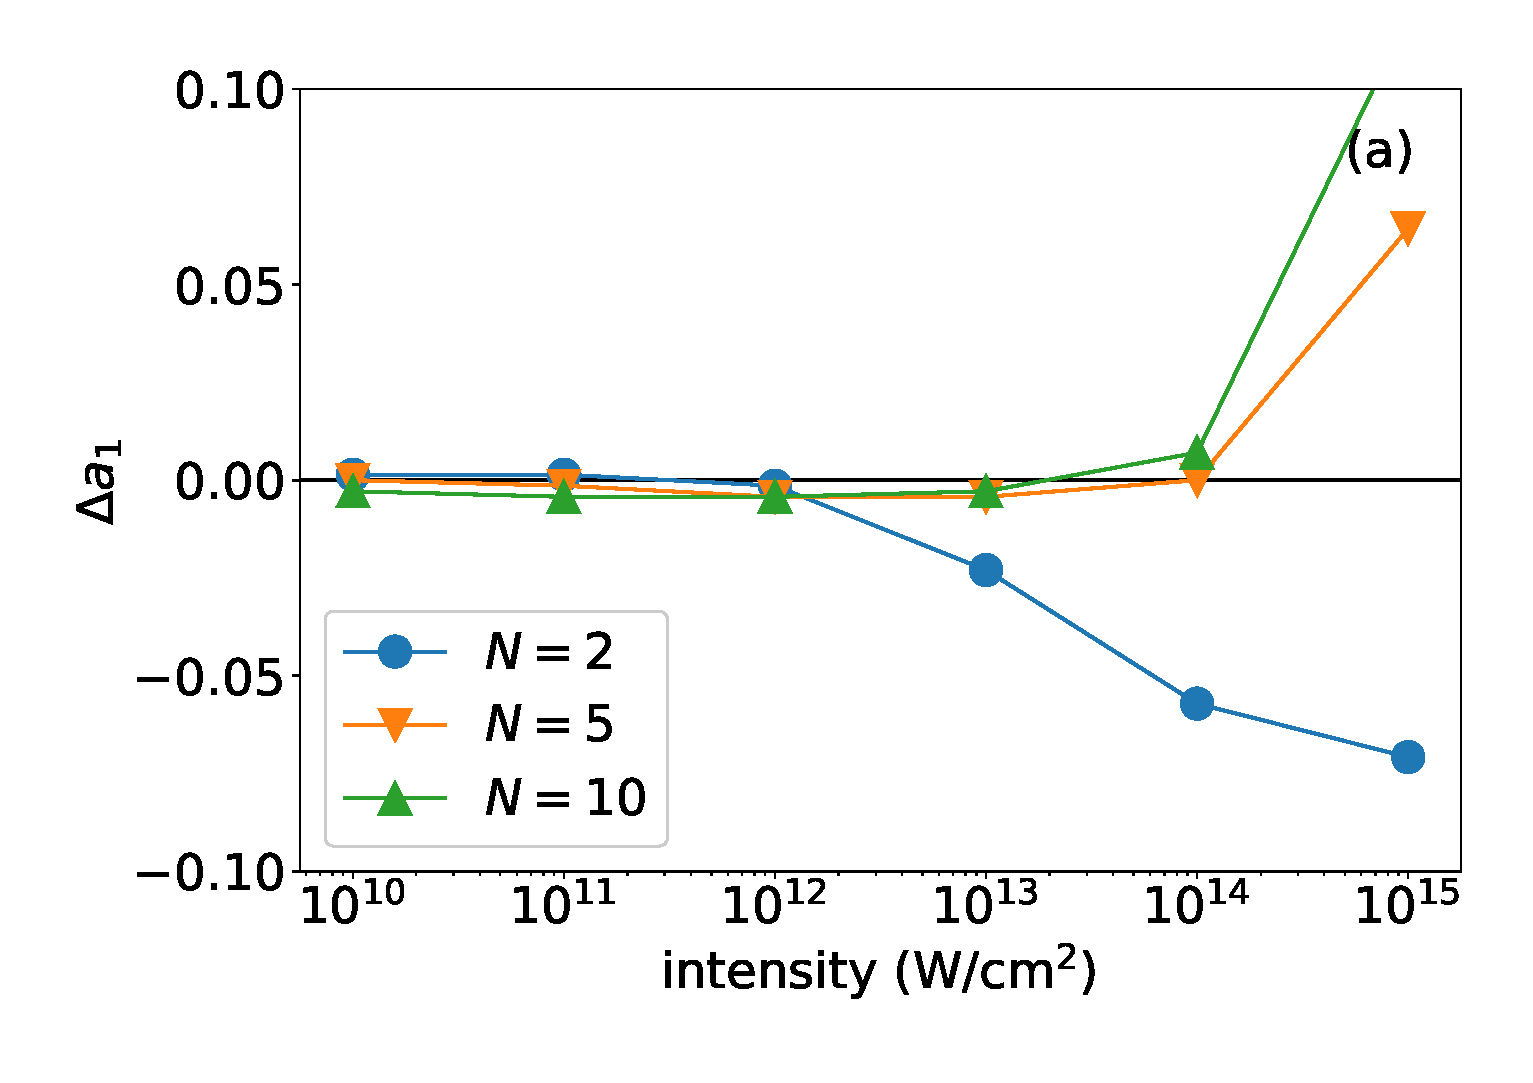
\includegraphics[width=0.32\linewidth]{figs/Photo_ionization/superpositions/Venzke_new_fig_3a.eps}
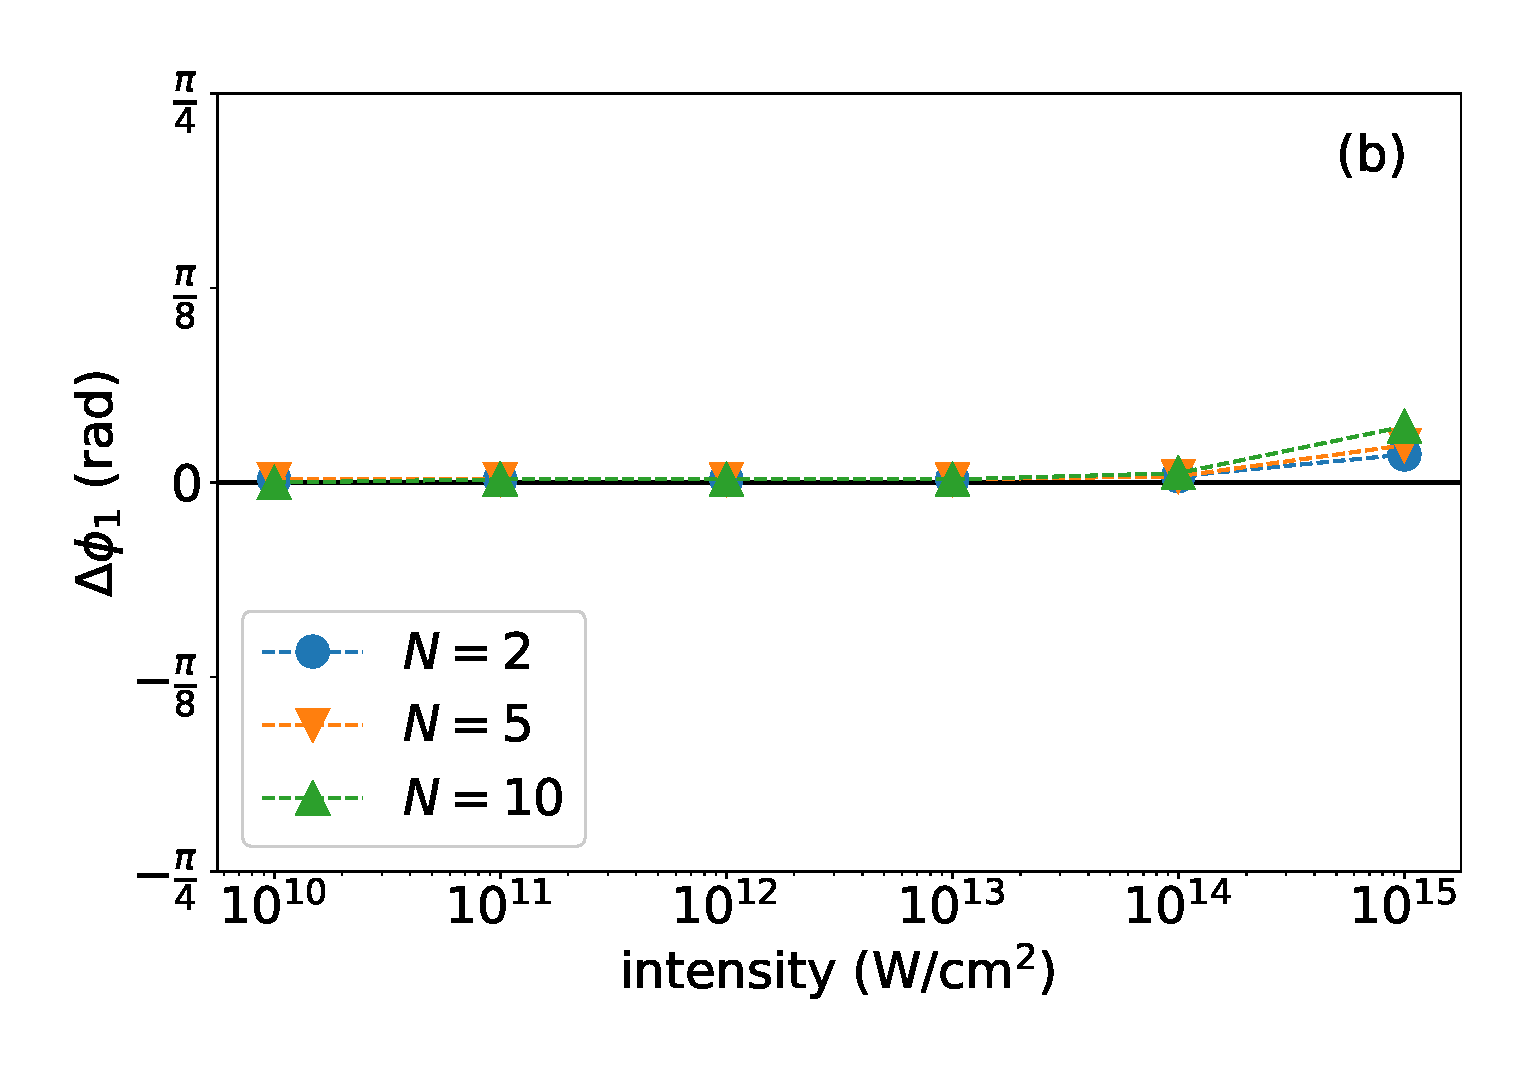
\includegraphics[width=0.32\linewidth]{figs/Photo_ionization/superpositions/Venzke_new_fig_3b.eps}
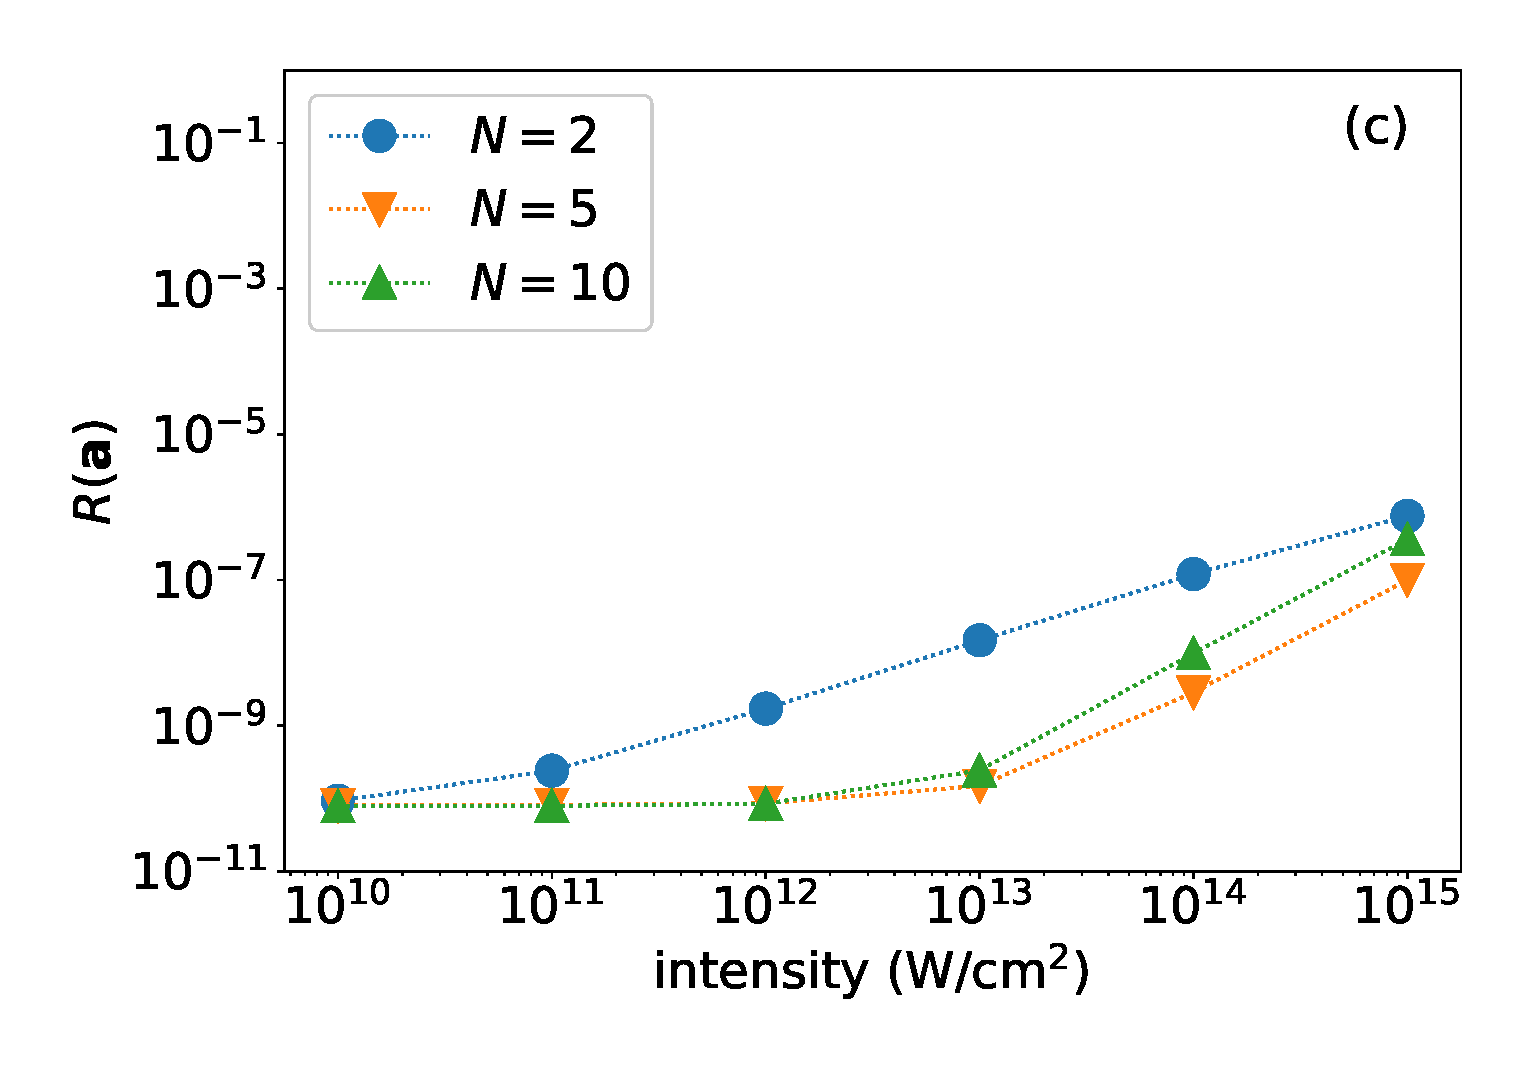
\includegraphics[width=0.32\linewidth]{figs/Photo_ionization/superpositions/Venzke_new_fig_3c.eps}\\
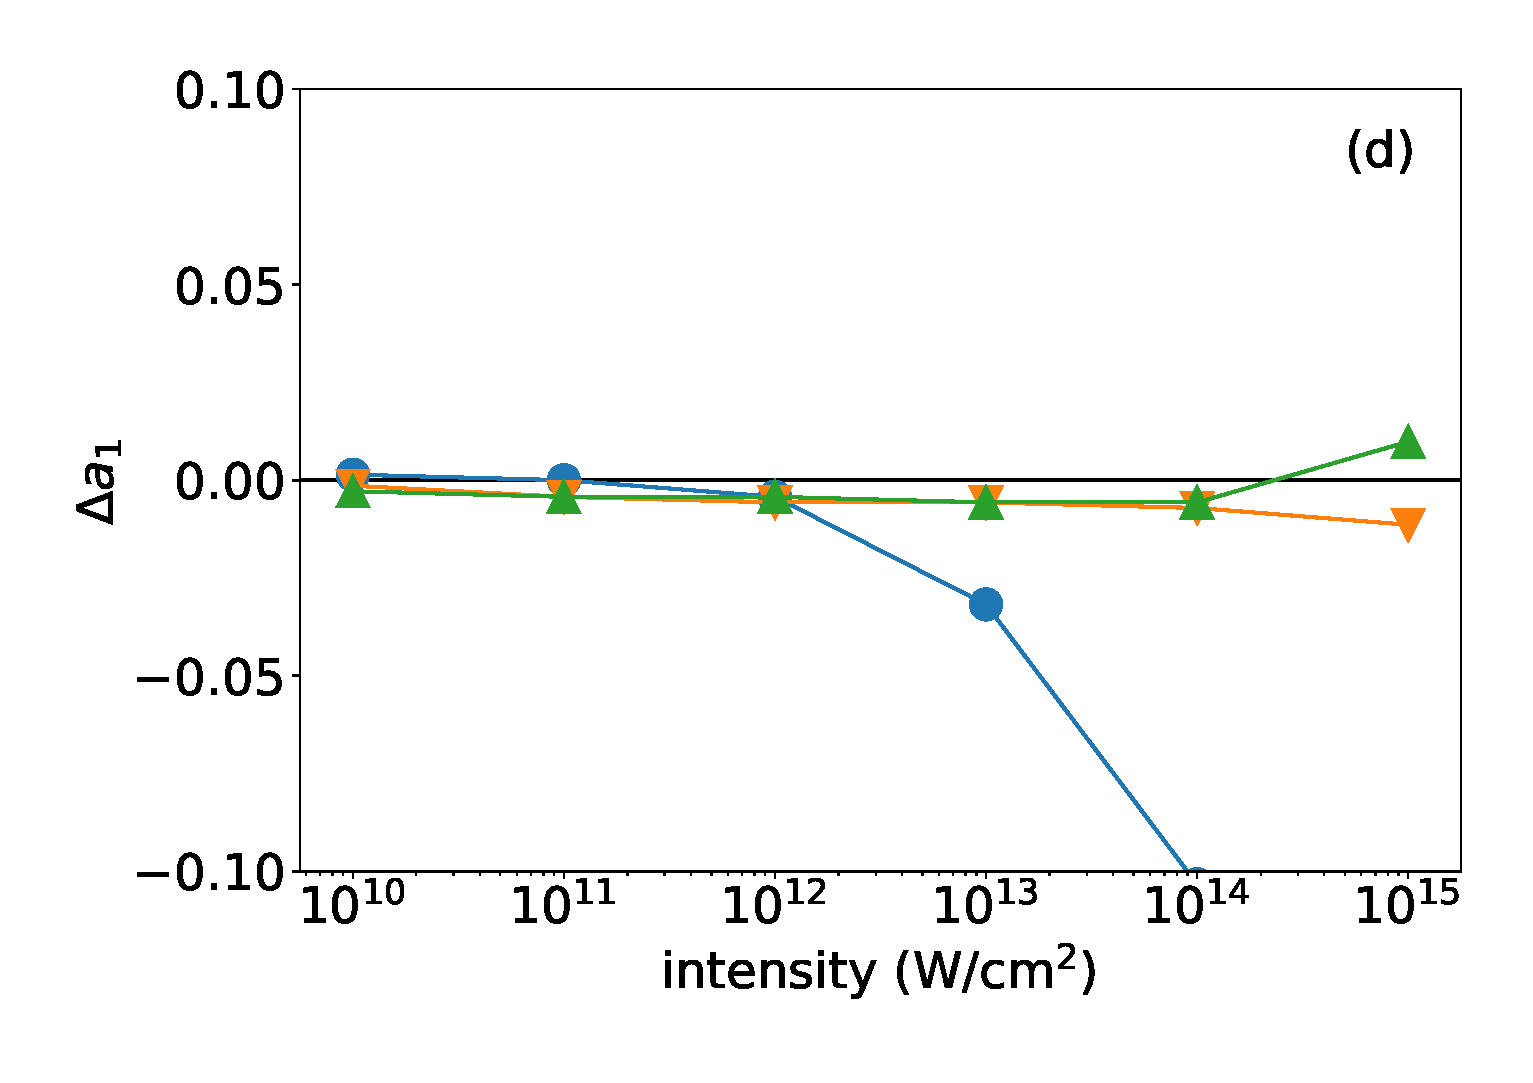
\includegraphics[width=0.32\linewidth]{figs/Photo_ionization/superpositions/Venzke_new_fig_3d.eps}
\includegraphics[width=0.32\linewidth]{figs/Photo_ionization/superpositions/Venzke_new_fig_3e.eps}
\includegraphics[width=0.32\linewidth]{figs/Photo_ionization/superpositions/Venzke_new_fig_3f.eps}
\caption{
Errors in amplitude (a, d) and phase (b, e) for the two-state reconstruction using PADs generated with laser pulses at two, five and ten cycle pulse duration. Also shown is the residual $R(\mathbf{a})$ (c, f).  The reconstructions are based on PADs at 20 time samples ($\Delta t=\tau/20$) using PADs in the full $x-y$ plane  (upper row) and photoelectron signals in forward-backward direction  (lower row). (Figure from \cite{venzke2021_wave})
} 
  \label{fig:resonant}
\end{figure*}

To demonstrate the reconstruction method the errors in reconstructing the amplitude (a, d) and phase (b, e) of the superposition state $(\ket{1s}+\ket{2p_+})/\sqrt{2}$ in helium atom as a function of peak intensity are shown in Fig.~\ref{fig:resonant}. The error is obtained via $\Delta a = a'-a$ where $a$ is the amplitude or phase of the original wave function and $a'$ is the corresponding amplitude or phase of the reconstructed wave function. The reconstruction is based on PADs taken at 20 time delays over one period of quantum beating $\tau = 2\pi / |E_{2p_1}-E_{1s}|$. Also shown are the final results of the minimization for $R(\mathbf{a})$  (panels (c) and (f)).

 Reconstructions of two cases are compared in which either the full PAD in the $x-y$ plane via signals at 6,285 equally spaced angles  (upper row) or only the signals in the forward-backward direction along the polarization axis of the probe pulse  (lower row) are used. The results in in the upper row show that  the reconstruction method reproduces the initial state up to peak laser intensities of about $10^{13}$ W/cm$^2$ if the full $x-y$ plane and 20 time samples are used. The increase of the errors at intensities larger than $10^{13}$ W/cm$^2$ indicates that higher-order processes  begin to contribute leading to the breakdown of the present second-order reconstruction method. For a two-state superposition just two amplitudes and the relative phase have to be determined. Using the full PAD with several thousand signals is oversampling for the reconstruction method. 
This is confirmed by the results for the reconstruction (d-f) using the PAD signals in forward-backward direction only. 

\begin{figure}[!ht]
\centering
\includegraphics[width=0.5\linewidth]{figs/Photo_ionization/superpositions/Venzke_new_fig_4.eps}
\caption{
Same as Fig.\ \ref{fig:resonant} but based on PADs at just two time delays. Errors in amplitude (filled symbols with solid lines) and phase (open symbols with dashed lines) are shown for using PADs in the full $x-y$ plane (blue squares) and in forward-backward direction (orange circles). (Figure from \cite{venzke2021_wave})
} 
  \label{fig:twosamples}
\end{figure}

Next, we have studied if one can limit the number of PAD samples over time. To this end, we present in Fig.\ \ref{fig:twosamples} the errors in amplitude and phase based on a reconstruction using just two PADs over one period of quantum beating $\tau = 2\pi / |E_{2p_1}-E_{1s}|$. If the full PAD in the $x-y$ plane is used (blue squares) the reconstruction method remains successful over the same intensity regime as before. However, when the available signals are limited to the forward-backward direction (orange circles), the data are insufficient for a one-to-one mapping between the initial state and the obtained photoelectron signal. Consequently, the reconstruction fails at nearly all peak laser intensities, since for just two time samples the normalization leads to a greater chance that multiple values for amplitudes and the relative phase produce a given signal.

Thus, for the basic case of equal population in a two-state superposition and probing with a pulse having a central frequency equal to the field-free energy difference of the state, our results show that the reconstruction method is successful for intensities in the perturbative regime up to $10^{13}$ W/cm$^2$. If the PADs can be measured over a broad range of angles probing at two times over one cycle of the probe pulse field is sufficient. In contrast, if only the forward-backward asymmetry signals are measured more time samples are needed.


\subsubsection{Impact of different pathways}

\begin{figure}[!ht]
\centering
\includegraphics[width=0.49\linewidth]{figs/Photo_ionization/superpositions/Venzke_new_fig_5a.eps}
\includegraphics[width=0.49\linewidth]{figs/Photo_ionization/superpositions/Venzke_new_fig_5b.eps}
\caption{Comparison of amplitude error for (a) two  and (b) five cycle probe pulse from calculations using full second order PT (blue), neglecting only the two-photon transition from the excited state (orange) and neglecting both the one-photon transition from the ground state and the two-photon amplitude from the excited state (green) in the reconstruction. (Figure from \cite{venzke2021_wave})
} 
  \label{fig:pathways}
\end{figure}

The reconstruction depends on the effective interference of at least two amplitudes to have a quantum beating. In the full reconstruction we consider the contributions from four pathways (one- and two-photon transitions from ground and excited states). It is interesting to ask which pathways contribute effectively besides the one-photon transition from the excited state. To study this question, we have deliberately neglected individual amplitudes in the reconstruction. In Fig.\ \ref{fig:pathways} we compare the results of these calculations with those of the full reconstruction (blue bars) based on the full $x-y$ plane and 20 time samples. We show the results for the amplitude error only and note that those for the phase error lead to the same conclusions.

We performed two set of test calculations: First, we utilized all amplitudes except the two-photon signal from the excited state (orange bars). Next, we have removed the one-photon signal from the ground state and the two-photon signal from the excited state from the reconstruction (green bars). Both transition amplitudes are expected to have an impact at ultrashort durations due to the broad bandwidth of the pulses. Indeed, we do see noticeable changes for the two-cycle data (a) while there appears to be insignificant impact for the five-cycle pulse (b) at all intensities.

For a two-cycle probe pulse, at intensities less than $10^{13}$ W/cm$^2$, the reconstruction without the two-photon amplitude from the excited state matches the full data (Fig.~\ref{fig:resonant}(a)). At higher intensities, the  results deviate which agrees with the expectation.  Removing also the one-photon transition from the ground state from the reconstruction causes the results to deviate from the full results at $10^{10}$ W/cm$^2$ and above $10^{13}$ W/cm$^2$. At the lowest intensity it is the one-photon signal from the ground state that provides a dominant contribution to the PAD, leading to the deviation at $10^{10}$ W/cm$^2$. At intensities above $10^{13}$ W/cm$^2$, the additional exclusion of the one-photon signal leads to a better reconstruction than for the full data and when the two-photon pathway from the excited state is neglected. This can indicate that inadvertently the two ultrashort amplitudes have an opposite effect on the reconstruction or that an even higher-order amplitude is more dominant than the lower-order processes.


\subsubsection{Variation of central frequency and population }
%%%%%%%%%%%%

\begin{figure}[!ht]
\centering
\includegraphics[width=0.49\linewidth]{figs/Photo_ionization/superpositions/Venzke_new_fig_6a.eps}
\includegraphics[width=0.49\linewidth]{figs/Photo_ionization/superpositions/Venzke_new_fig_6b.eps}
\includegraphics[width=0.49\linewidth]{figs/Photo_ionization/superpositions/Venzke_new_fig_6c.eps}
\includegraphics[width=0.49\linewidth]{figs/Photo_ionization/superpositions/Venzke_new_fig_6d.eps} 
\caption{
Amplitude (a, c) and phase (b, d) errors for ionization at a detuned photon frequency of $\omega=0.8\omega_0$ (upper row) and $\omega=1.2\omega_0$ (lower row). The reconstructions are based on full PADs in $x-y$ plane at 20 time delays. (Figure from \cite{venzke2021_wave})
} 
  \label{fig:detuned}
\end{figure}

So far, we have considered a special case with equal population in the two states and the central frequency tuned to the energy difference between the two field-free states. We will now study deviations from this special case. First, we consider a laser pulse detuned from the energy difference between the two equally populated states. We have calculated the photoelectron distribution at $E=\omega_E-|E_e|$, where $E_e$ is the energy of the excited $2p_1$-state. Given a sufficiently broad spectral range, i.e. sufficiently short pulse, the one-photon ground state signal (peaking at about $E = \omega_E-|E_g|$) at low intensities will interfere with the excited state signal creating the same quantum beating as before allowing for the reconstruction process to work. In Fig.~\ref{fig:detuned} we show the reconstruction results for a laser with central frequency of $\omega_E = 0.8\omega_0$ (upper row) and $\omega_E = 1.2\omega_0$ (lower row). 
The results lead to the same conclusion as for the resonant case, namely that the reconstruction method can be applied in the perturbative intensity regime up to $10^{13}$ W/cm$^2$.

\begin{figure}[!ht]
\centering
\includegraphics[width=0.5\linewidth]{figs/Photo_ionization/superpositions/Venzke_new_fig_7.eps}
\caption{
Amplitude and phase error for the reconstruction of an arbitrary unknown two-state superposition. Reconstruction is based on full PADs in $x-y$ plane at 20 time delays with a five-cycle probe pulse. (Figure from \cite{venzke2021_wave})
} 
  \label{fig:random_state}
\end{figure}

To show that the reconstruction works for a two-state superposition with arbitrary unknown amplitudes and phases, we have performed a `blindfold experiment' where the population of the states were chosen randomly. The random values were held unknown and were only accessed to obtain the final error at the end of the reconstruction procedure. We have used this approach in several calculations and for probe pulses of different duration, with results
leading to the same conclusion. As an example, one set of results for this `blindfold' experiment is presented in Fig.~\ref{fig:random_state}, showing that the reconstruction is successful with the same low errors as in the other cases studied.

\subsubsection{Detector accuracy and variation of laser parameters}

\begin{figure}[!ht]
\centering
\includegraphics[width=0.49\linewidth]{figs/Photo_ionization/superpositions/Venzke_new_fig_8a.eps}
\includegraphics[width=0.49\linewidth]{figs/Photo_ionization/superpositions/Venzke_new_fig_8b.eps}
\caption{
Comparison of (a) amplitude and (b) phase error for reconstruction using PADs at machine precision (blue) and with accuracy limited to 1\% and 10\%. (Figure from \cite{venzke2021_wave})
}
  \label{fig:detector}
\end{figure}

For the reconstructions so far
we have used results from TDSE calculations up to machine precision. Since detectors in experiment do not operate with the same precision we have studied how less accurate data may impact the success of the reconstruction. To this end, we have deliberately added random noise at a certain percentage level of the maximum signal in the PADs to the TDSE data. In Fig.\ \ref{fig:detector} we compare the results for the reconstruction with added noise at the  1\% and  10\% level with those at machine precision using the signals from the full $x-y$ plane and 20 time samples. It is seen that an accuracy of detection at the 1\% level is sufficient to reconstruct the wavefunction with similar error as in the full calculation with TDSE data at machine precision. Similar results and conclusions have been obtained for the other cases presented in Figs.\ \ref{fig:resonant} and \ref{fig:twosamples}. We expect that this limit can be achieved in a measurement.

\begin{figure}[!ht]
\centering
\includegraphics[width=0.49\linewidth]{figs/Photo_ionization/superpositions/Venzke_new_fig_9a.eps}
\includegraphics[width=0.49\linewidth]{figs/Photo_ionization/superpositions/Venzke_new_fig_9b.eps}
\caption{
Amplitude (a) and phase (b) error for variation of CEP only (blue squares with solid lines), intensity only (orange circles with dashed lines) and both CEP and intensity (green stars with dotted lines)
at peak intensity of  $10^{11}$ W/cm$^2$ and pulse duration of 2 cycles.  Reconstruction is based on full PADs in $x-y$ plane at 20 time delays. (Figure from \cite{venzke2021_wave})
} 
  \label{fig:noise}
\end{figure}

We have further considered variations in the laser parameters relevant for an application of the reconstruction method in an experiment. Typically, the peak intensity of the applied laser pulse may vary from shot to shot as well as over the interaction volume. Another parameter that is usually difficult to control is the carrier-to-envelope phase (CEP) of a laser pulse, specifically for ultrashort pulses. To study the impact on the reconstruction, CEP, peak intensity, and both CEP and peak intensity have been varied randomly within a certain percentage in the TDSE results. The results in Fig.~\ref{fig:noise} show that the reconstruction method still works well up to 10\% variation in both parameters before significant errors occur. Perhaps most surprising is the rather large acceptable tolerance in the CEP even for the shortest pulses, since CEP variations often lead to large changes in experimental observables. We assume that the shot to shot variation is `averaging out' over the various time delays leading to a quality in the reconstruction similar to fitting a linear regression to noisy data.

\subsubsection{Extension to superpositions of more than two states}

Finally, we consider the extension of the reconstruction method to a superposition of more than two states. The ionization scheme shown in Fig.\ \ref{fig:dynamic_visualization}(c) and (d) can be applied to each excited state in the superposition separately, taking the waves generated via one- and two-photon transitions from the ground state as reference. For the reconstruction measurement of PADs at separate energies for each excited state in the superposition is required. Based on PT results, residuals $R(\mathbf{a})$ (Eq.\ \ref{eqn:residual}) have been obtained, taking into account both final momenta to reconstruct the wave function.

\begin{figure}[!ht]
\centering
\includegraphics[width=0.48\linewidth]{figs/Photo_ionization/superpositions/Venzke_new_fig_10a.eps}
\includegraphics[width=0.48\linewidth]{figs/Photo_ionization/superpositions/Venzke_new_fig_10b.eps}\\
\includegraphics[width=0.48\linewidth]{figs/Photo_ionization/superpositions/Venzke_new_fig_10c.eps}
\includegraphics[width=0.48\linewidth]{figs/Photo_ionization/superpositions/Venzke_new_fig_10d.eps}

\caption{
Amplitude (a, c) and phase (b, d) errors for the reconstruction of the superposition $(\ket{1s}+\ket{2p_1}+\ket{3p_1})/\sqrt{3}$ in the helium atom (upper row: errors for $2p$-state, lower row: errors for $3p$-state).  (Figure from \cite{venzke2021_wave})
} 
  \label{fig:3-state}
\end{figure}

To test the extension of the method we have considered the helium atom in the $(\ket{1s}+\ket{2p_1}+\ket{3p_1})/\sqrt{3}$ superposition. A probe laser pulse at central photon energy tuned halfway between the $\ket{2p_1}$- and $\ket{3p_1}$-state and measurement of PADs at both $E=\omega-|E_{2p}|$ and $E=\omega-|E_{3p}|$ have been applied. The results of the reconstruction, based on PADs in the full $x-y$-plane taken at 20 time delays, are shown as function of peak intensity for different pulse durations in Fig.~\ref{fig:3-state}. The results show that a similar degree of accuracy in the reconstruction as for the two-state superposition is achieved within the same intensity limits. The example indicates that the present method may be extended to even more complex wave packets and electron dynamics. 

Extension of the reconstruction method to more complex superpositions will however require attention to the interference with the ground state signal and the increased dimensionality of the minimization space. Since the minimization process appears to be convex, a standard minimization algorithm, like stochastic gradient descent, may be sufficient for an efficient reconstruction. For each additional state in the interference scheme, the signal at the photoelectron energy chosen must include interference with at least one other state. This can be achieved if all transitions from the excited states interfere with that from the ground state by using a short pulse. If only longer pulses are available, coupling over many pairs of states reduces the required bandwidth for a reconstruction. Finally, due to the selection rules some initial states do not generate a signal in the $xy$-plane. In this case it may be required to utilize a full 4$\pi$-PAD for reconstruction of the corresponding superposition.

\subsection{Summary and outlook}
%%%%%%%%%%%%%%%%%

In this section we have studied the use of perturbation theory to reconstruct an atomic wave function representing ultrafast field-free charge migration. In the reconstruction scheme the photoelectron angular distributions obtained by ionizing an atom, prepared in a superposition of two or three states, are used. The electron dynamics are encoded in the PAD signal via interference of the ground and excited state ionization signals. Time delayed measurements allow for the extraction of all amplitudes and phases of the initial wavefuction that fully characterizes the charge migration. Results of applications based on TDSE calculations show that the reconstruction is highly accurate for probe pulse intensities below $10^{13}$ W/cm$^2$ while allowing for CEP (intensity) variations of 10\% (20\%) from shot to shot. Additionally, a detection accuracy for the PADs of about 1\% for a  reconstruction with small error is required.

These results may provide some basic guidelines for future experimental progress in imaging electron motion on its fundamental time scale via the detection of photoelectron angular distributions. However, the results also show that experimental challenges remain. Controlling the creation of ultrashort laser pulses, especially those with attosecond pulse duration, is a non-trivial task. For the current method to be applied, average values for intensity, CEP and pulse duration of the electric field of the probe pulse must be obtained and shot-to-shot variations must be limited up to a certain degree. Given the rate of advancement in attosecond laser pulse technology over the last decade, this level of pulse control may be, however, achieved in the coming years.


Additionally, precise knowledge of one- and two-photon transition dipoles is required to perform perturbation theory calculations for the target atom with high accuracy. Over the last decades several standard theoretical methods, such as multielectron theories, density functional theory or calculations using accurate single active electron potentials, have been developed to perform such calculations. As theoretical methods for bound and continuum wave functions further advance, the current and other reconstruction methods will become increasingly accurate.
% section wavefunction_reconstruction (end)

% chapter imaging_wave_packets_with_photoelectrons (end)
